%%%%%%%%%%%%%%%%%%%%%%%%%%%%%%%%%%%%%%%%%%%%%%%%%%%%%%%%%%%%%%%%%%%%%%
%%  disstemplate.tex, to be compiled with latex.		     %
%%  08 April 2002	Version 4				     %
%%%%%%%%%%%%%%%%%%%%%%%%%%%%%%%%%%%%%%%%%%%%%%%%%%%%%%%%%%%%%%%%%%%%%%
%%								     %
%%  Writing a Doctoral Dissertation with LaTeX at		     %
%%	the University of Texas at Austin			     %
%%								     %
%%  (Modify this ``template'' for your own dissertation.)	     %
%%								     %
%%%%%%%%%%%%%%%%%%%%%%%%%%%%%%%%%%%%%%%%%%%%%%%%%%%%%%%%%%%%%%%%%%%%%%


\documentclass[12pt]{report}	% The documentclass must be ``report''.

\usepackage{utdiss2}  		% Dissertation package style file.


%%%%%%%%%%%%%%%%%%%%%%%%%%%%%%%%%%%%%%%%%%%%%%%%%%%%%%%%%%%%%%%%%%%%%%
% Optional packages used for this sample dissertation. If you don't  %
% need a capability in your dissertation, feel free to comment out   %
% the package usage command.					     %
%%%%%%%%%%%%%%%%%%%%%%%%%%%%%%%%%%%%%%%%%%%%%%%%%%%%%%%%%%%%%%%%%%%%%%

\usepackage{amsmath,amsthm,amsfonts,amscd, amssymb} 
				% Some packages to write mathematics.
\usepackage{eucal} 	 	% Euler fonts
\usepackage{verbatim}      	% Allows quoting source with commands.
\usepackage{makeidx}       	% Package to make an index.
\usepackage{psfig}         	% Allows inclusion of eps files.
\usepackage{epsfig}         	% Allows inclusion of eps files.
%\usepackage{citesort}         	% 
\usepackage{url}		% Allows good typesetting of web URLs.
%\usepackage{draftcopy}		% Uncomment this line to have the
				% word, "DRAFT," as a background
				% "watermark" on all of the pages of
				% of your draft versions. When ready
				% to generate your final copy, re-comment
				% it out with a percent sign to remove
				% the word draft before you re-run
				% Makediss for the last time.

%The Rest of these are packages that I need for my thesis.
\usepackage{hyperref}
\usepackage{amsfonts}
\usepackage{graphicx}
\usepackage[english]{babel}
%\usepackage[
%backend=biber,
%style=ieee,
%sorting=ynt
%]{biblatex}
\usepackage{tikz}
\usepackage{algorithm}
\usepackage{algorithmicx}
\usepackage[noend]{algpseudocode}
\usepackage{geometry}
\usepackage{marginnote}
\usepackage{csquotes}

%\addbibresource{bibliography.bib}



\author{Matthew Alexander Denend}  	% Required

%Used email address as I STRONGLY preferred this as opposed 
%to physical address. 
\address{mdenend@gmail.com}  % Required

\title{Challenging Variants of the Collatz Conjecture}
                                                    % Required

%%%%%%%%%%%%%%%%%%%%%%%%%%%%%%%%%%%%%%%%%%%%%%%%%%%%%%%%%%%%%%%%%%%%%%
% NOTICE: The total number of supervisors and other members %%%%%%%%%%
%%%%%%%%%%%%%%% MUST be seven (7) or less! If you put in more, %%%%%%%
%%%%%%%%%%%%%%% they are put on the page after the Committee %%%%%%%%%
%%%%%%%%%%%%%%% Certification of Approved Version page. %%%%%%%%%%%%%%
%%%%%%%%%%%%%%%%%%%%%%%%%%%%%%%%%%%%%%%%%%%%%%%%%%%%%%%%%%%%%%%%%%%%%%

%%%%%%%%%%%%%%%%%%%%%%%%%%%%%%%%%%%%%%%%%%%%%%%%%%%%%%%%%%%%%%%%%%%%%%
%
% Enter names of the supervisor and co-supervisor(s), if any,
% of your dissertation committee. Put one name per line with
% the name in square brackets. The name on the last line, however,
% must be in curly braces.
%
% If you have only one supervisor, the entry below will read:
%
%	\supervisor
%		{Supervisor's Name}
%
% NOTE: Maximum three supervisors. Minimum one supervisor.
% NOTE: The Office of Graduate Studies will accept only two supervisors!
% 
%
\supervisor
	[Scott Aaronson]
	{Marienus Heule}

%%%%%%%%%%%%%%%%%%%%%%%%%%%%%%%%%%%%%%%%%%%%%%%%%%%%%%%%%%%%%%%%%%%%%%
%
% Enter names of the other (non-supervisor) members(s) of your
% dissertation committee. Put one name per line with the name
% in square brackets. The name on the last line, however, must
% be in curly braces.
%
% NOTE: Maximum six other members. Minimum zero other members.
% NOTE: The Office of Graduate Studies may restrict you to a total
%	of six committee members.
%
%
%\committeemembers
%	[Erwin Schr\"odinger]
%	[Albert Einstein]
%	[Charles Townes]
%	{Arthur Schawlow}

%%%%%%%%%%%%%%%%%%%%%%%%%%%%%%%%%%%%%%%%%%%%%%%%%%%%%%%%%%%%%%%%%%%%%%

\previousdegrees{B.S.}
     % The abbreviated form of your previous degree(s).
     % E.g., \previousdegrees{B.S., MBA}.
     %
     % The default value is `B.S., M.S.'

%\graduationmonth{...}      
     % Graduation month, either May, August, or December, in the form
     % as `\graduationmonth{May}'. Do not abbreviate.
     %
     % The default value (either May, August, or December) is guessed
     % according to the time of running LaTeX.

%\graduationyear{...}   
     % Graduation year, in the form as `\graduationyear{2001}'.
     % Use a 4 digit (not a 2 digit) number.
     %
     % The default value is guessed according to the time of 
     % running LaTeX.

%\typist{...}       
     % The name(s) of typist(s), put `the author' if you do it yourself.
     % E.g., `\typist{Maryann Hersey and the author}'.
     %
     % The default value is `the author'.


%%%%%%%%%%%%%%%%%%%%%%%%%%%%%%%%%%%%%%%%%%%%%%%%%%%%%%%%%%%%%%%%%%%%%%
% Commands for master's theses and reports.			     %
%%%%%%%%%%%%%%%%%%%%%%%%%%%%%%%%%%%%%%%%%%%%%%%%%%%%%%%%%%%%%%%%%%%%%%
%
% If the degree you're seeking is NOT Doctor of Philosophy, uncomment
% (remove the % in front of) the following two command lines (the ones
% that have the \ as their second character).
%
\degree{MASTER OF SCIENCE IN COMPUTER SCIENCE}
\degreeabbr{M.S. Comp.Sci.}

% Uncomment the line below that corresponds to the type of master's
% document you are writing.
%
%\masterreport
\masterthesis


%%%%%%%%%%%%%%%%%%%%%%%%%%%%%%%%%%%%%%%%%%%%%%%%%%%%%%%%%%%%%%%%%%%%%%
% Some optional commands to change the document's defaults.	     %
%%%%%%%%%%%%%%%%%%%%%%%%%%%%%%%%%%%%%%%%%%%%%%%%%%%%%%%%%%%%%%%%%%%%%%
%
%\singlespacing
%\oneandonehalfspacing

%\singlespacequote
\oneandonehalfspacequote

\topmargin 0.125in	% Adjust this value if the PostScript file output
			% of your dissertation has incorrect top and 
			% bottom margins. Print a copy of at least one
			% full page of your dissertation (not the first
			% page of a chapter) and measure the top and
			% bottom margins with a ruler. You must have
			% a top margin of 1.5" and a bottom margin of
			% at least 1.25". The page numbers must be at
			% least 1.00" from the bottom of the page.
			% If the margins are not correct, adjust this
			% value accordingly and re-compile and print again.
			%
			% The default value is 0.125"

		% If you want to adjust other margins, they are in the
		% utdiss2-nn.sty file near the top. If you are using
		% the shell script Makediss on a Unix/Linux system, make
		% your changes in the utdiss2-nn.sty file instead of
		% utdiss2.sty because Makediss will overwrite any changes
		% made to utdiss2.sty.

%%%%%%%%%%%%%%%%%%%%%%%%%%%%%%%%%%%%%%%%%%%%%%%%%%%%%%%%%%%%%%%%%%%%%%
% Some optional commands to be tested.				     %
%%%%%%%%%%%%%%%%%%%%%%%%%%%%%%%%%%%%%%%%%%%%%%%%%%%%%%%%%%%%%%%%%%%%%%

% If there are 10 or more sections, 10 or more subsections for a section,
% etc., you need to make an adjustment to the Table of Contents with the
% command \longtocentry.
%
%\longtocentry 



%%%%%%%%%%%%%%%%%%%%%%%%%%%%%%%%%%%%%%%%%%%%%%%%%%%%%%%%%%%%%%%%%%%%%%
%	Some math support.					     %
%%%%%%%%%%%%%%%%%%%%%%%%%%%%%%%%%%%%%%%%%%%%%%%%%%%%%%%%%%%%%%%%%%%%%%
%I USED MY OWN HERE.
%
%	Theorem environments (these need the amsthm package)
%
%% \theoremstyle{plain} %% This is the default
\newtheorem{theorem}{Theorem}[section]
\newtheorem{corollary}{Corollary}[theorem]
\newtheorem{lemma}[theorem]{Lemma}

%\theoremstyle{definition}
%\newtheorem{definition}{Definition}[section]
%\newtheorem{question}{Question}[section]

\newcommand{\Mod}[1]{\ (\mathrm{mod}\ #1)}
\newcommand{\Col}[1]{\mathrm{Col}(#1)}
\newcommand{\ColMod}[3]{\mathrm{Col}_{\text{mod}}(#1,#2,#3)}
%\newtheorem{thm}{Theorem}[section]
%\newtheorem{cor}[thm]{Corollary}
%\newtheorem{lem}[thm]{Lemma}
%\newtheorem{prop}[thm]{Proposition}
%\newtheorem{ax}{Axiom}

%\theoremstyle{definition}
%\newtheorem{defn}{Definition}[section]

%\theoremstyle{remark}
%\newtheorem{rem}{Remark}[section]
%\newtheorem*{notation}{Notation}

%\numberwithin{equation}{section}


%%%%%%%%%%%%%%%%%%%%%%%%%%%%%%%%%%%%%%%%%%%%%%%%%%%%%%%%%%%%%%%%%%%%%%
%	Macros.							     %
%%%%%%%%%%%%%%%%%%%%%%%%%%%%%%%%%%%%%%%%%%%%%%%%%%%%%%%%%%%%%%%%%%%%%%
%
%	Here some macros that are needed in this document:


\newcommand{\latexe}{{\LaTeX\kern.125em2%
                      \lower.5ex\hbox{$\varepsilon$}}}

\newcommand{\amslatex}{\AmS-\LaTeX{}}

\chardef\bslash=`\\	% \bslash makes a backslash (in tt fonts)
			%	p. 424, TeXbook

\newcommand{\cn}[1]{\texttt{\bslash #1}}

\makeatletter		% Starts section where @ is considered a letter
			% and thus may be used in commands.
\def\square{\RIfM@\bgroup\else$\bgroup\aftergroup$\fi
  \vcenter{\hrule\hbox{\vrule\@height.6em\kern.6em\vrule}%
                                              \hrule}\egroup}
\makeatother		% Ends sections where @ is considered a letter.
			% Now @ cannot be used in commands.

\makeindex    % Make the index

%%%%%%%%%%%%%%%%%%%%%%%%%%%%%%%%%%%%%%%%%%%%%%%%%%%%%%%%%%%%%%%%%%%%%%
%		The document starts here.			     %
%%%%%%%%%%%%%%%%%%%%%%%%%%%%%%%%%%%%%%%%%%%%%%%%%%%%%%%%%%%%%%%%%%%%%%

\begin{document}

\copyrightpage          % Produces the copyright page.


%
% NOTE: In a doctoral dissertation, the Committee Certification page
%		(with signatures) is BEFORE the Title page.
%	In a masters thesis or report, the Signature page
%		(with signatures) is AFTER the Title page.
%
%	If you are writing a masters thesis or report, you MUST REVERSE
%	the order of the \commcertpage and \titlepage commands below.
%
\commcertpage           % Produces the Committee Certification
			%   of Approved Version page (doctoral)
			%   or Signature page (masters).
			%		20 Mar 2002	cwm

\titlepage              % Produces the title page.



%%%%%%%%%%%%%%%%%%%%%%%%%%%%%%%%%%%%%%%%%%%%%%%%%%%%%%%%%%%%%%%%%%%%%%
% Dedication and/or epigraph are optional, but must occur here.      %
%%%%%%%%%%%%%%%%%%%%%%%%%%%%%%%%%%%%%%%%%%%%%%%%%%%%%%%%%%%%%%%%%%%%%%
%
\begin{dedication}
\index{Dedication@\emph{Dedication}}%
Dedicated to my late mother, who passed away earlier this year, yet never
let her three battles with cancer stop her from endlessly loving her sons and
her husband.
\end{dedication}


\begin{acknowledgments}		% Optional
\index{Acknowledgments@\emph{Acknowledgments}}%
I want to give a huge thank you to both of my advisors for this project: Scott Aaronson and Marijn Heule. \par
Scott Aaronson came to UT Austin from MIT in fall 2016. I knew that I wanted to write a Master's Thesis from pretty much the time I started my Master's Degree, and I heard he might be a great person to work with. We come from very different backgrounds. He is well-renowned for his work in Theoretical Quantum Computing. I came into UT's CS program with virtually no Math/CS theory background, as my undergrad degree was in Electrical Engineering. At one point, he suggested that I talk to Marijn Heule, and hence, this project was born. I got a chance to witness firsthand the enthusiasm that Scott has for CS and Math theory, and it's no wonder that Scott has done so much work in Theoretical Computer Science... he just keeps going and going! This entire project would not have been possible without him and he is as much, if not more, of an author of this Thesis as I am. I'm also deeply thankful to him for his support as I had to go through the challenge of losing my mom.\par
Marijn Heule became an Assistant Research Professor at UT in fall 2017. He was a Research Scientist at UT Austin when I first met him. Marijn is a master at SAT Solving, and is famous for his proof of the Boolean Pythagorean Triples problem that was the largest proof ever at the time at 100 TB. Much like Scott, Marijn has a great deal of enthusiasm for mathematical problems. This entire project is originally Marijn's idea, so I am thankful that he had this idea, and I am very happy to have written a Thesis with such a cool topic. Without his advice and direction and his many read-overs and edits, this Thesis would have not been possible to finish, so he is as much, if not more, of an author of this Thesis as I am. I am also deeply thankful of the support he gave me as I had to go through the challenge of losing my mom.\par
When Scott and Marijn first met each other, they raced each other to solve several proofs related to this project: Scott by hand, Marijn using computation. I happened to be in the middle of it all, unable to keep up with the blazing speed of these two brilliant minds. It took me some time but I can now confidently read through these original thoughts that Scott and Marijn had and understand most of them much better now then when they first occurred. \par
I am forever indebted to these two men and can only hope to someday achieve the greatness and brilliance of them. \par
I am also thankful for the many friends that I have made along the way towards finishing this Thesis, especially those who gave me support as I had to deal with the loss of my mom. There are far too many to list, but you know who you are. From my time here in Austin, I have made many friends that I want to keep for many years to come.
\end{acknowledgments}


% The abstract is required. Note the use of ``utabstract'' instead of
% ``abstract''! This was necessary to fix a page numbering problem.
% The abstract heading is generated automatically.
% Do NOT use \begin{abstract} ... \end{abstract}.
%
\utabstract
\index{Abstract}%
\indent
%Should not exceed 350 words. Looks like I have a good amount.
The Collatz Conjecture (also known as the $3x+1$ problem) is simple to explain, yet proving that all positive integers following the Collatz map must converge to 1 has eluded mathematicians for over half a century. Aaronson and Heule are exploring solving the Collatz Conjecture using an approach involving string rewrite systems: Aaronson transformed the Conjecture into a string rewrite system and Heule applied parallel SAT solvers on instances of this system. Similar approaches have been applied successfully to other mathematical problems.\par
We started looking into simpler, but also challenging variants of the conjecture. This thesis defines some of these variants and investigates easily provable as well as very hard variants. We study the hardness of unsolved variants by computing the number of rewrite steps needed up to 1 billion. Our hardness prediction method suggests that proving termination of the challenging variants should be considerably easier compared to solving the original conjecture.
\tableofcontents   % Table of Contents will be automatically
                   % generated and placed here.

%\listoftables      % List of Tables and List of Figures will be placed
\listoffigures     % here, if applicable.



%%%%%%%%%%%%%%%%%%%%%%%%%%%%%%%%%%%%%%%%%%%%%%%%%%%%%%%%%%%%%%%%%%%%%%
% Actual text starts here.					     %
%%%%%%%%%%%%%%%%%%%%%%%%%%%%%%%%%%%%%%%%%%%%%%%%%%%%%%%%%%%%%%%%%%%%%%
%
% Including external files for each chapter makes this document simpler,
% makes each chapter simpler, and allows for generating test documents
% with as few as zero chapters (by commenting out the include statements).
% This allows quicker processing by the Makediss command file in case you
% are not working on a specific, long and slow to compile chapter. You
% can even change the chapter order by merely interchanging the order
% of the include statements (something I found helpful in my own
% dissertation).
%
\chapter{Introduction} \label{sec:introduction}
%Introduction: First sentence: Computers have been very powerful applications for many things, but they don't work for seemingingly simple problems.

%Second sentence: Does  there  exist  a  program  that  can  determine  if  an  arbitrary  program  with arbitrary input will terminate? 

%Will a given program on any input always terminate? Be careful here.

%Turing  proved  that  the  halting  problem  is  undecidable,  because: replace because with in other words, this means that ... make it less formal. 

%As a given problem for all inputs. Make sure this is clear, and resend him another copy of this first paragraph in the near future.

%Algorithm 1 is Classical, 4 is generalization throughout the thesis.  Delete Algorithm 2, and 3 and move Algorithm 4 from section 2 to section 1, use that here.

%Algorithm 1: Collatz Conjecture Recursion. Algorithm 4: A generalization of the Collatz Conjecture Recursion. The Collatz Conjecture halts for some variants of alg. 4. Call Alg 3/4 subscript _{\text{mod}}. Text for names, italic for variables.

%Since  the  Collatz  Conjecture  seems  to  be  quite  difficult  to  prove: replace with Since  the  Collatz  Conjecture  has been challenging to prove, instead o

%This thesis also follows an attempt that Heule and Aaronson have devised to attemptto solve the Collatz Conjecture with computers: replace first attempt with an approach

% At a high level, it involves taking a completely reworked formulation: replace with reformulation.
% It is important that the central termination property is clear. This is not the case. You now describe three variants: 1) a given program on an arbitrary input; 2) a given program on any input (Collatz); and 3) a given problem with no input (Hello World). The thesis only deals with 2) so I would make sure that all the text only discusses instances of 2).
%HERE IS NEW
Computers have been successfully applied to many complex problems, such as those in finance, healthcare, and the Internet. However, computers still struggle with seemingly simple problems. Consider whether a given program on any input will always terminate. One can easily show that certain programs will always halt. For example, we can easily show a program that takes an integer input $x$, computes $y=x+1$, prints $y$, then halts, will always terminate. Nevertheless, there exist simple programs that are much harder to determine if they always terminate. Algorithm~\ref{alg:ColR} is such an example. Will this program always return 1 for any positive integer $N$, causing it to halt? This problem is a reformulation of the Collatz Conjecture. \par
\begin{algorithm} 
\caption{The Collatz Conjecture Sequence, $\Col{N}$}
\label{alg:ColR} 
\begin{algorithmic}[1]
    \If{$N \leq 1$} \Return $N$ 
    \EndIf
    \If {$N \equiv 0 \Mod{2}$} \Return $\Col{N/2}$
    \EndIf
    \State \Return $\Col{3N + 1}$ 
\end{algorithmic}
\end{algorithm}
We know from Turing that no program exists to determine if an arbitrary program with arbitrary input can halt~\cite{Turing1936}, but that does not exclude the possibility of a program that determines if specifically Algorithm~\ref{alg:ColR} halts. However, no program has been found to show that all positive integer inputs for Algorithm~\ref{alg:ColR} will halt, even though this problem can be explained to an elementary grade student. The problem has been extensively analyzed, according to surveys by Lagrias~\cite{2003mathLagrais}~\cite{2006mathLagrias}, yet no proof has been found. Further, empirical evidence suggests that the Collatz Conjecture is true. According to a website maintained by Eric Roosendahl~\cite{EricRoose}, all numbers up to $87 \cdot 2^{60}$, or about $10^{20}$, have been tried as $N$ in Algorithm~\ref{alg:ColR}, and have converged to 1. \par
Since the Collatz Conjecture has been challenging to prove, we propose another supposedly simpler variant of it. Can we prove that the code in Algorithm \ref{alg:ColSP}, where $A = \{1\}$, and $b = 8$ ($\ColMod{N}{\{1\}}{8}$ is shorthand for this problem), always terminates for any positive integer $N$? Even though this program seems to be easier, we do not have a program showing this variant always terminates either! \par
\begin{algorithm} 
\caption{A Collatz Conjecture Variant $\ColMod{N}{A}{b}$}
\label{alg:ColSP} 
\begin{algorithmic}[1]
    \If{$(N \leq 1) \vee (N \equiv a_1  \Mod{b}) \vee \ldots \vee (N \equiv a_s \Mod{b})$ } \Return $N$
    \EndIf
    \If {$N \equiv 0 \Mod{2}$} \Return $\ColMod{N/2}{A}{b}$
    \EndIf
    \State \Return $\ColMod{3N+1}{A}{b}$ 
\end{algorithmic}
\end{algorithm}
One of the goals of this Thesis is to try and determine how hard certain variants of the Collatz Conjecture are to solve. A contribution of this thesis is that it uses empirical data to try and find trends of hardness for difficult variants, and compare these trends to the hardness of solving the whole Collatz Conjecture. This thesis also follows an approach that Heule and Aaronson have devised to attempt to craft a program to determine if Algorithm~\ref{alg:ColR} always halts~\cite{HeuleAaronson}. At a high level, it involves taking a completely reworked formulation of Algorithm~\ref{alg:ColR} and using known techniques that, if certain conditions are met, the reworked formulation can be shown to terminate for any positive integer input. The formulation requires SAT solvers, string rewrite systems, and a technique called matrix interpretation, all topics which will be covered briefly in this paper as background. This thesis also investigates a rewrite system that Aaronson crafted, and we believe that, if Aaronson's system is found to terminate for all input, the Collatz Conjecture holds. We analyze properties of this rewrite system and the variants from before are investigated with this rewrite system as well.\par
The rest of this thesis is outlined as follows: Chapter~\ref{sec:defns} introduces definitions that will be used throughout the paper. Chapter~\ref{sec:alttercdns} defines several Collatz Conjecture variants, including both solvable ones and unsolved ones, including $\ColMod{N}{\{1\}}{8})$. Chapter~\ref{sec:subhrdnspred} analyzes the difficulty of these variants using algebra. Chapter ~\ref{sec:SRSandSAT} provides a brief background on SAT Solvers and String Rewrite Systems, how SAT solvers can be used to prove termination of them, describes Aaronson's rewrite system that Heule tried to use with matrix interpretation and SAT solving to prove, and the results of this approach. Finally, chapter~\ref{sec:hardnessrewriterules} investigates hardness of solving the same variants covered in chapter~\ref{sec:subhrdnspred}, but derived from Aaronson's rewrite system instead.

\chapter{Definitions} \label{sec:defns}
We will use the following terms throughout the paper to talk about the $3x+1$ problem:
\begin{itemize}
    \item $\boldsymbol{3x+1}$\textbf{ mapping}: A one step application of $Col(N)$ to some input number $N$.
    \item $\boldsymbol{3x+1}$\textbf{ sequence}: Define this as follows: 
    \begin{align*}
        x_0 = x &= \text{ initial input number} \\
        x_{i+1} &= \begin{cases} 
        x_{i}/2 &\text{ if $x_i$ is even} \\
        3 x_{i} + 1 &\text{ if $x_i$ is odd} \\
        \end{cases}
    \end{align*}
    This sequence can continue for arbitrarily large values of $i$, but we are only interested in following the sequence until $x_i$ for some $i$ is 1, as any value after 1 follows the $1 \rightarrow 4 \rightarrow 2 \rightarrow 1$ cycle indefinitely.
    \item \textbf{Collatz Variant:} When we say ``Collatz Variant,'' we use Algorithm~\ref{alg:ColSP}, which was defined in the introduction. The shorthand for this will be $\ColMod{N}{A}{b}$, where $A = \{a_1 \ldots a_s\}$ is all of the bases that cause termination of the algorithm. Note that for all $a \in A$, $0 \le a < b$, and $A = \emptyset$ is the same as Algorithm~\ref{alg:ColR}.
    \item \textbf{Collatz Variant a:} The vast majority of our analyis is when $b = 8$, so when we say Collatz Variant a, it is shorthand for $\ColMod{N}{A}{8}$ where $A = \{a\}$. Note this notation only allows for a singleton set $A$, so when we list multiple variants, like Collatz Variants, 1, 5, and 7, we mean the three variants $\ColMod{N}{\{1\}}{8}$, $\ColMod{N}{\{5\}}{8}$, and $\ColMod{N}{\{7\}}{8}$. 
    \item \textbf{Collatz Variant $\boldsymbol{\{a_1,a_2\}}$:} A Collatz Variant with a set of 2 or larger elements in $A$ will always use set notation. Example: Collatz Variant $\{5,7\}$ means $\ColMod{N}{\{5,7\}}{8}$.
    \item \textbf{Collatz String Rewrite System(SRS):} Created by Aaronson~\ref{HeuleAaronson}, and introduced in chapter~\ref{sec:SRSandSAT}, along with background of string rewrite systems, this is used in the latter portion of this paper as an alternative way of expressing the Collatz Conjecture.
    \item \textbf{Collatz Subproblem:} Modifying the rewrite rules in the Collatz SRS by modifying/removing certain rules. This is used in chapter~\ref{sec:hardnessrewriterules} to explore modifications of the Collatz SRS that are akin to Collatz Variants.
    \item \textbf{Number of bits:} For an input number $x$, we say that, written in binary, it has $m$ bits.
\end{itemize}


\chapter{Alternative Termination Conditions} \label{sec:alttercdns}
 This chapter explores some of the possible Collatz Variants. Before we investigate them, we define a graph paradigm that transforms the $3N+1$ problem into directed graphs that depict the flow for all input numbers modulo base $b$, where $b$ is a power of 2. Using this paradigm, we can show that some variants are easily provable. However, others are not.
\section{Base \textit{b} Collatz Graph Definition} \label{subsec:colgraph}
Define $G_b=(V,E)$ to be a ``Base $b$ Collatz Graph'', where $b = 2^k$, and $k$ is nonnegative. Choosing a power of 2 for $b$ allows us to easily reason with binary numbers, which is useful for both several proofs in this chapter and the Collatz SRS that we will discuss starting in Chapter~\ref{sec:SRSandSAT}. \hl{$V$ has $b$ vertices in it, where each vertex is labeled a unique integer in the interval $[0, b-1]$. We say that a number $N$ is visiting vertex $v \in V$ if and only if $N \equiv v \Mod{b}$ for vertex $v$ labeled with integer $v$. Out of convenience, note that we use $v$ as a vertex and integer interchangeably in this paper. %\par

%, when we refer to vertex $v$, we are referring both to the vertex $v \in V$, and a number $v$, such that $N$ visiting the vertex labelled $v$ means $N \equiv v \Mod{b}$.

% We often use the vertex label $v$ and numbers interchangeably, so if we say ``node $v$'', we are talking about $v \Mod{b}$ and the vertex $v \in V$ interchangeably. This is done out of conveneince.
%This thesis uses the term ``node $v$'' as shorthand to correspond to the number $v$ in $v \Mod{b}$, as opposed to ``vertex $v$'' which corresponds to the actual vertex of the graph. 

Let $N$ be an input number, and $N_1$ the result of applying the $3N+1$ mapping to $N$. $E = V \times V$ is a set of directed edges, where, for nodes $u, v \in V$, $(u,v) \in E$ if and only if $N_i \equiv u \Mod{b}$ and $N_{i+1} \equiv v \Mod{b}$ for some $N$ and $N_1$.}

\section{Base \textit{b} Collatz Graph Lemmas}
This section contains some lemmas that are used throughout this chapter. First, we start with a lemma about the number of node transitions in any Collatz Base $b$ Graph $G_b$.
\begin{lemma}
\label{lem:numOutEdges}
Given a Collatz Base $b$ Graph, for all $v \in V$, if node $v$ is even, then it has two outgoing edges. Otherwise, if node $v$ is odd, then it has only one outgoing edge.
\end{lemma}
\begin{proof}
\hl{Take some number $N$ that is visiting node $v$, and consider $N$ in binary. First, let us consider the case where node $v$ is even. When we divide by 2, we just remove the lowest 0 bit from $N$ to get $N_{1}$. The bit at index $k-1$ of $N_{1}$ can be either a 0 or a 1, allowing for two options for even nodes. \par
Now, let $N$ visit an odd node $v$. Multiplying $N$ by 3 and adding 1 will give us a $N_1$ where the binary string for it grows at least one bit longer than $N$, since $3\cdot N = 2 \cdot N + N$, and $2N$ in binary is shifting the bits of $N$ one index to the left, then adding a 0 bit to the least significant bit. This gives us only one option for the least significant $k$ bits, meaning $N_1$ can only visit one node, and only one such outgoing edge from $v$ exists.}
\end{proof}
Now, we have a couple of important properties about cycles that exist in any Collatz Base $b$ Graph, and the fact that these cycles cannot continue indefinitely. First, we introduce the ``0 cycle'' lemma.
\begin{lemma}
\label{lem:zeroCycle}
For any Collatz Base $b$ Graph (where $b$ is a positive power of 2), a self-loop occurs on a 0 node. This cycle cannot continue indefinitely.
\end{lemma}
\begin{proof}
Assume we have an input number $N$ such that $N \equiv 0 \Mod{b}$. This means that the $k$ least significant bits are all 0. Apply the $3N+1$ mapping once to this string. We remove a 0 from the end, since we divide the input number by 2. We now look at the new number $N_1$ and the $k$ least significant bits. The $k-1$ least significant bits are all 0. But what is the value of the bit in the most significant of the $k$ lowest bits of $N_1$? If it is a 0, then $N_1 \equiv 0 \Mod{b}$, and we have a self-loop. \par
To show that the self loop cannot continue indefinitely: every time we follow the self-loop, remove a 0. Since we also know that $N > 1$ in order for the algorithm to continue running, we also know that at least one binary digit is a 1. So as we continue dividing by 2 and removing bits that are 0, we eventually reach, after $i$ visits to node 0, a point where the least $k$ significant bits are $1000\ldots 0$, meaning $N_i$ is visiting node $b/2$ instead, ending the cycle.
\end{proof}
Now, we introduce another important lemma about cycles: the fact that we will always have a cycle between nodes $b-2$ and $b-1$, and it cannot continue indefinitely.
\begin{lemma}
\label{lem:oneConsumption}
 For any Collatz Base $b$ Graph, a cycle between exists between nodes $b-2$ and $b-1$. This cycle cannot continue indefinitely.
\end{lemma}
\begin{proof}
In this proof, we will show first that a $b-1 \rightarrow b-2 \rightarrow b-1$ cycle exists, and second, that this cycle cannot continue indefinitely; more precisely, that some number congruent modulo to $b-2 \Mod{b}$, after division by 2, actually becomes congruent modulo to $b/2-1 \Mod{b}$ instead. We will prove this using long multiplication in binary. \par
%x NEEDS to remain x here, make it equal to some number N
Let $x$ be a arbitrary number\footnote{\hl{Normally, we use the notation $N$ to denote an arbitrary number in the $3N+1$ sequence, but we mean $N_i$ to mean the $i$\textsuperscript{th} number in the $3N+1$ sequence, whereas in this proof, we have $x_j$ to denote the $j$\textsuperscript{th} bit of $x$. Hence, we use variables $x$ and $y$ instead of $N$ and $N_1$.}} congruent modulo to $b-1 \Mod{b}$. We want to express $x$ in binary, so let $x$ have $m$ bits. We know that since $x$ is congruent modulo to $b-1 \Mod{b}$, all bits from indices 0 to $k-1$ are 1. Let $x_j$ denote the $j$\textsuperscript{th} bit of $x$, $k \leq j \leq m$. These bits are unknown. Let $1_{+1}$ correspond to the adding of 1 after multiplying by 3, which is added to the least significant bit of $x$. Let $c_j$ denote the unknown carry for the $j$\textsuperscript{th} addition of bits. Let $y$ be the result after $3x+1$ is computed, and let index $j$ of $y$ be the same index as $x$. The multiplication is referenced in Figure~\ref{fig:mul}. \par
\begin{figure}
\begin{tabular}{*{16}c}%{c*{15}{@{\,}c}}
 & & $ x_{n}$  & $ x_{n-1}$  & \ldots & $ x_{j+1}$  & $ x_{j}$  & \ldots & $ x_{k+1}$  & $ x_{k}$  & 1 & 1 & \ldots & 1 & 1 & 1 \\
$\times$ & & & & & & & & & & & & & & 1 & 1 \\
\hline
\tiny ${\scriptscriptstyle c_{n+2}}$ & ${\scriptscriptstyle c_{n+1}}$ & ${\scriptscriptstyle c_{n}}$ & ${\scriptscriptstyle c_{n-1}}$ & & ${\scriptscriptstyle c_{j+1}}$ & ${\scriptscriptstyle c_{j}}$ & & ${\scriptscriptstyle c_{k+1}}$ & \tiny 1 & \tiny 1 &  \tiny 1 & &  \tiny 1 & \tiny 1 & \\
  & & $ x_{n}$  & $ x_{n-1}$  & \ldots & $ x_{j+1}$  & $ x_{j}$  & \ldots & $ x_{k+1}$  & $ x_{k}$  & 1 & 1 & \ldots & 1 & 1 & 1 \\
  + & $ x_{n}$  & $ x_{n-1}$  & $ x_{n-2}$  & \ldots & $ x_{j}$  & $ x_{j-1}$  & \ldots & $ x_{k}$  & 1 & 1 & 1 & \ldots & 1 & 1 & $1_{+1}$  \\
  \hline
  $ y_{n+2}$  & $ y_{n+1}$  & $ y_{n}$  & $ y_{n-1}$  & \ldots & $ y_{j+1}$  & $ y_{j}$  & \ldots & $ y_{k+1}$  & $ y_{k}$  & 1 & 1 & \ldots & 1 & 1 & 0 
\end{tabular}
\caption{The long multiplication corresponding to $3x + 1$. Note how, in the addition step, the $1_{+1}$ is in place of a zero, and the addition is just $x + 2x + 1$.}
\label{fig:mul}
\end{figure}
As mentioned in lemma~\ref{lem:numOutEdges}, multiplication of a binary number $x$ by 3 is just $x + 2x$, and $2x$ is just placing all bits of $x$ one index to the left, adding a 0 bit at the newly vacant spot. In the multiplication we show in Figure~\ref{fig:mul}, we write this but replace the new least significant 0 bit of $2x$ with the special $1_{+1}$ bit, allowing us to perform $3x+1$ with just one addition instead of two. \par
Notice that all bits in the resulting binary number $y$ from indices 0 to $k-1$ are 1, except for index 0, which is 0. This is because all bits of $y$, save the least significant bit, are computed by adding $1+1$ and carrying over the 1 from the previous addition. As a result, $y$ is congruent modulo to $b-2 \Mod{b}$, meaning an edge from node $b-1 \Mod{b}$ to node $b-2 \Mod{b}$ exists in our graph.\par
When we divide $y$ by 2, we just remove the least significant 0 bit from $y$, decreasing the indices of all bits in $y$ by 1. Hence, bit $y_k$ is now in position $k-1$. If $y_k$ is 1, our number is now congruent modulo to $b-1 \Mod{b}$. This means an edge also exists from node $b-2 \Mod{b}$ to node $b-1 \Mod{b}$, proving the existence of the $b-2 \rightarrow b-1 \rightarrow b-2$ cycle. \par
Now we show that this cycle will always eventually terminate. This happens when, after dividing a number congruent modulo to $b-2 \Mod{b}$ by 2, bit $y_{k-1}$ is 0. So we need to show this eventually occurs for any positive integer $x$. There are two cases for this:
\begin{enumerate}
    \item Some bit in $x$ is 0. Let $x_j$ be the least significant bit of $x$ that is 0 (all bits which have indices lower than $j$ are 1). Look back at Figure~\ref{fig:mul}, and replace $x_j = 0$, and have all bits at indices less than $j$ be 1. After taking the $3x+1$ step, all bits of $y$ between 1 and $j-1$ will be 1, since for each bit, we add $1 + 1$ and carry over a 1. However, when we get to index $j$, we add $1 + 0$ plus a carry of 1, making bit $y_j = 0$. Since after we divide by 2 we move all bits one index to the right, bit $y_j$ now moves to index $j-1$. We repeat this process a total of $j-k+1$ times. After this, the 0 bit will be in position $y_{k-1}$, making $y$ congruent modulo to $b/2 - 1 \Mod{b}$ instead, breaking the cycle.
    \item No bit in $x$ is 0. In this case, again looking at Figure~\ref{fig:mul}, all bits in $y$ from indices 1 to $m$ will be 1. However, bit $y_{m+1} = 0$, because $y_{m+1} = c_{m+1} + x_{m} + x_{m+1}$, and $c_{m+1} = 1$ and $x_{m} = 1$, but $x_{m+1} = 0$. Since bit $y_{m+1} = 0$ we move it over one index to index $m$ after dividing by 2. We then follow case 1, where $j = m$, and hence, the cycle also breaks in this case.
 \end{enumerate}
 Hence, no input number can follow the $b-2 \rightarrow b-1 \rightarrow b-2$ cycle indefinitely. 
\end{proof}
We introduce one more lemma that shows that cycles where the magnitude of divisions by 2 outweigh the magnitude of multiplications by 3. We call this the ``even node dominance lemma''.
\begin{lemma}
\label{lem:EvenDom}
Given a cycle in any Collatz Base $b$ Graph $G$, let $V_{e}$ be the set of even nodes in the cycle, and $V_{o}$ be the set of odd nodes. If $2^{|V_e|} > 3^{|V_o|}$, then the cycle cannot continue indefinitely.
\end{lemma}
\begin{proof}
Let $2^{|V_e|} > 3^{|V_o|}$ \hl{and $j=|V_e| + |V_o|$. Let $N$ be visiting a node $v$ in the cycle, and assume $N$ will run through the cycle at least once without terminating, implying no number between $N$ and $N_j$ inclusive is 1, and that $N_j$ visits the same node $v$ as $N$ did.} We visited $|V_e|$ vertices in the cycle, so we divided $N$ by $2^{|V_e|}$ after one trip around the cycle. We also visited $|V_o|$ vertices in the cycle, each time multiplying by 3, and overall, multiplied $N$ by about $3^{|V_o|}$.\footnote{We also added one each time we visit an odd node, but this is asymptotically insignificant compared to multiplying by 3 or dividing by 2, so we ignore it in this proof.}\par
Hence, after we visited the cycle once, we computed $N_{j} \approx \frac{3^{|V_o|}}{2^{|V_e|}}N$. Since $2^{|V_e|} > 3^{|V_o|}$, $N_{j} < N$. Therefore, one of two things must happen:
\begin{enumerate}
\item $N$ eventually becomes 1, which means the cycle no longer can be repeated.
\item The cycle is eventually broken.
\end{enumerate}
In both cases, the cycle cannot continue indefinitely.
\end{proof}
\section{Base 4 Collatz Graph and Variants} \label{subsec:base4graph}
\hl{In this section, we build a simple example of a Base $b$ Collatz Graph:  $G_4$. We chose $G_4$ because we can prove that $\ColMod{N}{A}{4}$ terminates for any nonempty $A \subseteq \{0,1,2,3\}$. In $G_4$, there are 4 different nodes: one for each integer between 0 and 3. When determining which node $v$ input number $N$ visits, we look at the lowest 2 bits of $N$, since $4= 2^2$. For example, $N \equiv 0\Mod{4}$ has 00 as the 2 least significant bits, whereas $N \equiv 2\Mod{4}$ has 10 as its 2 least significant bits.}
 \subsection{Base 4 Collatz Graph Construction} \label{subsubsec:proofbase4graph}
Figure~\ref{fig:base_4_graph} shows \hl{$G_4$. We describe the construction in this subsection. We start by describing the transitions for even nodes, then the transitions for odd nodes. Assume, in all cases, that a number $N$ is written in binary. First, the transitions for even nodes:}
\begin{figure}
    \centering
    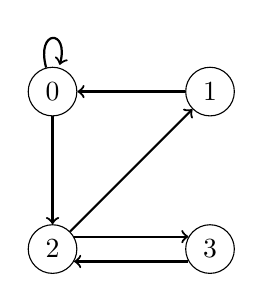
\begin{tikzpicture}
    \node[shape=circle,draw=black] (A) at (0,2) {0};
    \node[shape=circle,draw=black] (B) at (2,2) {1};
    \node[shape=circle,draw=black] (C) at (0,0) {2};
    \node[shape=circle,draw=black] (D) at (2,0) {3};
    \path  (A) edge [loop above, thick] (A);
    \path [->] (B) edge [thick] (A);  
    \path [->] (A) edge [thick] (C);  
    \path [->] (C) edge [thick] (B);  
    \path [->] (C.30) edge [thick] (D.150);  
    \path [->] (D.210) edge [thick] (C.-30);  
    \end{tikzpicture}
    \caption{The Base 4 Collatz Graph, $G_4$. There are 4 nodes, each one corresponding to a value mod 4.}
    \label{fig:base_4_graph}
\end{figure}

\begin{itemize}
    \item \hl{$N$ visiting node 0 means $N$ ends with binary string ``00''. Removing the last 0 bit of $N$ leaves either ``00'', meaning $N_1$ visits node 0 again, or ``10'', meaning $N_1$ visits node 2 instead.} 
    \item \hl{$N$ visiting node 2 means $N$ ends with binary string ``10''. Removing the last 0 bit of $N$ leaves either ``01'', meaning $N_1$ visits node 1, or ``11'', meaning $N_1$ visits node 3.}
\end{itemize}
Now, the transitions for odd nodes. Let $x_2$ and $x_3$ be unknown bits:
\begin{itemize}
    \item \hl{$N$ visiting node 1 means $N$ ends with binary string ``01''.  Multiplying this by 3 and adding 1 results in $N_1$ ending with ``$x_200$'', so $N_1$ visits node 0.}
    \item \hl{$N$ visiting node 3 means $N$ ends with binary string ``11''.  Multiplying this by 3 and adding 1 results in $N_1$ ending with ``$x_3x_210$'', so $N_1$ visits node 2.}
\end{itemize}
\subsection{Base 4 Collatz Variants} \label{subsubsec:base4variants}
We introduced the Base 4 case for nodes because we can prove that we need to visit all of the nodes in this graph, which is equivalent to saying that each of the Collatz Variants, $\ColMod{N}{A}{4}$ terminates for nonempty $A \subseteq \{0,1,2,3\}$, and for any input number $N$. 
\begin{theorem}
$\ColMod{N}{A}{4}$ terminates for nonempty $A \subseteq \{0,1,2,3\}$.
\end{theorem}
\begin{proof}
\hl{Assume that no $3N+1$ sequence described in this proof reaches 1, otherwise $\ColMod{N}{A}{4}$ terminates trivially for any $A$.} We will start with proving that $\ColMod{N}{\{2\}}{4}$ will terminate for any input number $N$, because the 2 node is central to the Base 4 graph.  \par
\begin{lemma}
\label{lem:collatzSubTwoModFour}
$\ColMod{N}{\{2\}}{4}$ terminates for any $N$.
\end{lemma} 
\begin{proof}
We use the graph to help in this proof. An equivalent question is this: Can we show that node 2 must be visited for all input numbers? To show that this is the case, we have to show that all other nodes must visit node 2.
\begin{itemize}
    \item 2: \hl{If the input number $N$ is visiting node 2, we are already done.}
    \item 3: \hl{If the input number $N$ is visiting node 3, then after the $3N+1$ mapping is applied to $N$, $N_1$ is now visiting node 2.}
    \item 1 and 0: \hl{Let $N$ be visiting node 1. $N_1$ visits node 0 after applying the $3N+1$ mapping once. To show $N_{1+j}$ must leave node 0}, we use lemma~\ref{lem:zeroCycle} (the ``0 cycle'' lemma) for $b = 4$, \hl{and $N_{1+j}$ will visit node 2 after $j$ more applications of the $3N+1$ mapping, both causing $\ColMod{N}{\{2\}}{4}$ to terminate.}
\end{itemize}
Since all other nodes must visit node 2, it means that for all $N$, $\ColMod{N}{\{2\}}{4}$ terminates.
\end{proof} \par

\begin{lemma}
\label{lem:collatzSubOneModFour}
$\ColMod{N}{\{1\}}{4}$ terminates for any $N$.
\end{lemma}
\begin{proof}
We use lemma~\ref{lem:collatzSubTwoModFour} \hl{to show that node 2 must be visited, meaning that for any input number $N$, $N_i \equiv 2 \Mod{4}$ after $i$ steps. Then we use lemma}~\ref{lem:oneConsumption} \hl{to show that the cycle between nodes 2 and 3 cannot continue indefinitely, so after $j$ more steps, $N_{i+j}$ visits node 1, proving termination of this variant.}
\end{proof}
\begin{lemma}
\label{lem:collatzSubZeroModFour}
$\ColMod{N}{\{0\}}{4}$ terminates for any $N$.
\end{lemma}
\begin{proof}
Given lemma~\ref{lem:collatzSubOneModFour}, we know after $i$ steps $N_i$ must visit node 1, and given lemma~\ref{lem:numOutEdges}, an odd node can only have one outgoing edge, so $N_{i+1}$ visits node 0.
\end{proof}
\begin{lemma}
\label{lem:collatzSubThreeModFour}
$\ColMod{N}{\{3\}}{4}$ terminates for any $N$.
\end{lemma}
\begin{proof}
Given the ``even node dominance lemma'',~\ref{lem:EvenDom}, \hl{the $2 \rightarrow 1 \rightarrow 0 \rightarrow \ldots \rightarrow 2$ cycle cannot continue forever because, if we assume that the 0 node never self-cycles, $2^2 > 3^1$. The 0 self-cycle makes even nodes dominate even more. So an input number $N$ in the $2 \rightarrow 1 \rightarrow 0 \rightarrow \ldots \rightarrow 2$ cycle must, after $i$ steps, visit node 3, causing $\ColMod{N}{\{3\}}{4}$ to terminate.}
\end{proof}
Since all of these lemmas hold, it follows that any singleton set from $A \subseteq \{0,1,2,3\}$ causes $\ColMod{N}{A}{4}$ to terminate. Also, by definition of Algorithm~\ref{alg:ColSP}, any larger size sets for $A$ also terminate as larger set sizes add more termination conditions. So any nonempty set $A$ will cause $\ColMod{N}{A}{4}$ to terminate for any input $N$.
\end{proof}
\section{Base 8 Collatz Graph and Variants} \label{subsec:base8graphsubpblms}
After proving $\ColMod{N}{A}{4}$ terminates for any nonempty base set $A$ and input number $N$, we decided to see what would happen if we expanded to $k = 3$ bits. We have not been able to prove all variants of $\ColMod{N}{A}{8}$ for all nonempty sets $A$. This will motivate further computation undertaken in Chapter~\ref{sec:subhrdnspred}, as we try to determine how hard figuring out these unproven variants are. Figure~\ref{fig:base_8_graph} shows the base 8 graph. There are 8 different nodes, since $8 = 2^3$.
\begin{figure}
    \centering
    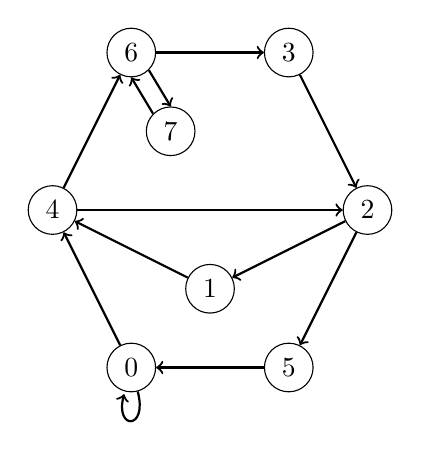
\begin{tikzpicture}
    \node[shape=circle,draw=black] (A) at (1,0) {0};
    \node[shape=circle,draw=black] (B) at (2,1) {1};
    \node[shape=circle,draw=black] (C) at (4,2) {2};
    \node[shape=circle,draw=black] (D) at (3,4) {3};
    \node[shape=circle,draw=black] (E) at (0,2) {4};
    \node[shape=circle,draw=black] (F) at (3,0) {5};
    \node[shape=circle,draw=black] (G) at (1,4) {6};
    \node[shape=circle,draw=black] (H) at (1.5,3) {7};
    \path  (A) edge [loop below, thick] (A);
    \path [->] (A) edge [thick] (E);  
    \path [->] (B) edge [thick] (E);  
    \path [->] (C) edge [thick] (B);  
    \path [->] (C) edge [thick] (F);  
    \path [->] (D) edge [thick] (C);  
    \path [->] (E) edge [thick] (C);  
    \path [->] (E) edge [thick] (G);  
    \path [->] (F) edge [thick] (A);  
    \path [->] (G) edge [thick] (D);  
    \path [->] (G.-45) edge [thick] (H.90);  
    \path [->] (H.135) edge [thick] (G.-90);  
    \end{tikzpicture}
    \caption{The Base 8 Collatz Graph, $G_8$. There are 8 nodes, each one corresponding to a value mod 8.}
    \label{fig:base_8_graph}
\end{figure}

\subsection{Base 8 Collatz Graph Construction} \label{subsubsec:base8proof}
Like $G_4$ before, we show how to construct $G_8$. We examine the even nodes first. In this case, there are four different nodes: 0, 2, 4, and 6. Using lemma~\ref{lem:numOutEdges}, each vertex has two different transitions, depending on what the next bit to the left of the 3 bits after removing the least significant 0. % \item \hl{$N$ visiting node 2 means $N$ ends with binary string ``10''. Removing the last 0 bit of $N$ leaves either ``01'', meaning $N_1$ visits node 1, or ``11'', meaning $N_1$ visits node 3.}


\begin{itemize}
    \item $N$ visiting node 0 means $N$ ends with binary string ``000''. Removing the last 0 bit of $N$ leaves either ``000'', meaning $N_1$ loops to node 0; or ``100'', meaning $N_1$ visits node 4 instead.
    \item $N$ visiting node 2 means $N$ ends with binary string ``010''. Removing the last 0 bit leaves either ``001'', meaning $N_1$ visits node 1; or ``101'', meaning $N_1$ visits node 5.
    \item $N$ visiting node 4  means $N$ ends with binary string ``100''. Removing the last 0 bit leaves either ``010'', meaning $N_1$ visits node 2; or ``110'', meaning $N_1$ visits node 6.
    \item $N$ visiting node 6 means $N$ ends with binary string ``110''. Removing the last 0 bit leaves either ``011'',  meaning $N_1$ visits node 3, or ``111'',  meaning $N_1$ visits node 7.
\end{itemize}
Now, the odd nodes. Let $x_3$ and $x_4$ be unknown bits.
%    \item \hl{$N$ visiting node 1 means $N$ ends with binary string ``01''.  Multiplying this by 3 and adding 1 results in $N_1$ ending with ``$x_200$'', so $N_1$ visits node 0.}
\begin{itemize}
    \item $N$ visiting node 1 means $N$ ends with binary string ``001''. Multiplying this by 3 and adding 1 results in $N_1$ ending with ``$100$'', so $N_1$ visits node 4.
    \item $N$ visiting node 3 means $N$ ends with binary string ``011''. Multiplying this by 3 and adding 1 results in $N_1$ ending with ``$x_3010$'',  so $N_1$ visits node 2.
    \item $N$ visiting node 5 means $N$ ends with binary string ``101''. Multiplying this by 3 and adding 1 results in $N_1$ ending with ``$x_4x_3000$'', so $N_1$ visits node 0.
    \item $N$ visiting node 7 means $N$ ends with binary string ``111''. Multiplying this by 3 and adding 1 results in $N_1$ ending with ``$x_4x_3110$'', so $N_1$ visits node 6.
\end{itemize}
\subsection{Base 8 Collatz Graph Cycle Analysis} \label{subsubsec:cycleanalysis}
Since we do not have proofs for all Collatz Variants $\ColMod{N}{A}{8}$, we analyzed whether certain cycles can last indefinitely. \hl{We have found that all simple cycles of $G_8$ can be proven to not last indefinitely. However, showing that some combinations of these simple cycles cannot continue forever is much more difficult to do.}\par
\hl{We tie in interesting Collatz Variants to these analyses. We start with smaller cycles and work our way into longer cycles, as well as combinations of them.}
\begin{itemize}
    \item The 0 self-cycle, ($0  \rightarrow \ldots$) cannot continue forever, as per lemma~\ref{lem:zeroCycle}.
    \item The $6 \rightarrow 7 \rightarrow 6$ cycle cannot continue forever as per lemma~\ref{lem:oneConsumption}.
    \item The $4 \rightarrow 2 \rightarrow 1 \rightarrow 4$ cycle cannot continue forever, as even nodes dominate ($2^2 > 3$), so according to lemma~\ref{lem:EvenDom}, this cycle cannot last forever.
    \item $4 \rightarrow 2 \rightarrow 5 \rightarrow 0  \rightarrow \ldots \rightarrow 4$ cycle:  Even nodes dominate, even without any 0 self-cycles ($2^3 > 3$), so according to lemma~\ref{lem:EvenDom}, this cycle cannot continue forever. \hl{We can also combine this cycle with the $4 \rightarrow 2 \rightarrow 1 \rightarrow 4$ cycle, and since both cycles cause input numbers to decrease, the combination of these two cycles must visit a new node to prevent the number from converging to 1. The only other choice is node 6, so this argument is used to prove Collatz Variant 6 must terminate.}
    \item $4 \rightarrow 6 \rightarrow 3 \rightarrow 2 \rightarrow 1 \rightarrow 4$ cycle: There are three different variations of this cycle. We have a proof for only one of them:
\begin{itemize}
  \item No transition allowed from $4 \rightarrow 2$: The following theorem explains this case.
  \begin{theorem} Aaronson '17: The $4 \rightarrow 6 \rightarrow 3 \rightarrow 2 \rightarrow 1 \rightarrow 4$ cycle cannot continue indefinitely.
  \end{theorem}
  \begin{proof}
    If we start some number $N$ such that $N \equiv 4\Mod{8}$, and follow the $4 \rightarrow 6 \rightarrow 3 \rightarrow 2 \rightarrow 1 \rightarrow 4$ cycle once, we turn $N$ into $(9N+20)/8 = \frac{9}{8}(N+20)-20$. If we were to repeat the cycle $k$ times, we would turn $N$ into $\frac{9}{8}^k(N+20)-20$. This quantity must be an integer for all $k$ if the cycle is to continue forever. However, $N+20$ will only have a finite number of factors of 8, so the cycle must terminate.
  \end{proof}
  \item Transition allowed between $4 \rightarrow 2$: This creates a conflict between two different cycles: one that causes growth by approximately a factor of $9/8$ ($4 \rightarrow 6 \rightarrow 3 \rightarrow 2 \rightarrow 1 \rightarrow 4$), and another that causes the cycle to decay by a factor of $4/3$ ($4 \rightarrow 2 \rightarrow 1 \rightarrow 4$). Even though we can prove that both of these cycles terminate independently, it has been a challenge to show that the combination of them cannot continue indefinitely, as we cannot prove that one cycle must stop transitioning to the other. Hence, no proof, by hand or machine, is known that we must break out of this combination of cycles, by visiting either node 5 or 7. A proof that this combination of cycles must be broken would prove termination of Collatz Variant $\{5,7\}$, which we explore in Chapter~\ref{sec:subhrdnspred}.
  \item Building on the prior point, we can also consider visits to the node 7 as well in this cycle. This adds the $6 \rightarrow 7 \rightarrow 6$ cycle to the already challenging two cycle case. If we can't prove that the smaller combination of cycles $4 \rightarrow 6 \rightarrow 3 \rightarrow 2 \rightarrow 1 \rightarrow 4$ and $4 \rightarrow 2 \rightarrow 1 \rightarrow 4$ cannot terminate, it would be far more difficult to add a third cycle, even though all three cycles must terminate individually. A proof of this cycle would solve Collatz Variant 5, also explored in Chapter~\ref{sec:subhrdnspred}.
\end{itemize}
\item $4 \rightarrow 6 \rightarrow 3 \rightarrow 2 \rightarrow 5 \rightarrow 0 \rightarrow \ldots \rightarrow 4$ cycle: There are three different variations to showing this cycle cannot continue forever: keeping both nodes 1 and 7 omitted, or omitting one node or the other. Adding in both nodes yields the entire base 8 graph. The variant where both 1 and 7 are omitted is proven, the other two are not.
    \begin{itemize}
        \item Strictly following this cycle, no changes: assuming no zero-cycles, there are 4 distinct even nodes in this cycle, and 2 distinct odd nodes. $2^4 > 3^2$, so according to the ``even node dominance lemma'',~\ref{lem:EvenDom}, this cycle cannot continue forever. The nodes that must be visited to break this cycle are either 1 or 7, so this is a proof that Collatz Variant $\{1,7\}$ terminates.
        \item Allowing 7 but avoiding 1: Like variant $\{5,7\}$, we have two conflicting cycles: the $6 \rightarrow 7 \rightarrow 6$ cycle which cause the number to grow by approximately $\frac{3}{2}$ every time it takes this cycle, and the base cycle $4 \rightarrow 6 \rightarrow 3 \rightarrow 2 \rightarrow 5 \rightarrow 0 \rightarrow \ldots \rightarrow 4$ that reduces it by approximately $\frac{16}{9}$, depending on number of zero self cycles. These two cycles are interesting in that they clash the fastest growing part of the graph: the $6 \rightarrow 7 \rightarrow 6$ cycle, and the fastest decaying part of the graph: the 0 self-cycle, followed by two more even numbers. We are also not aware of a proof for this case either. Such a proof that these two cycles cannot continue combined forever would be equivalent to proving termination of Collatz Variant 1. We present analysis of hardness of this cycle in Chapter~\ref{sec:subhrdnspred}.
        \item Allowing 1 but avoiding 7: Adding back in node 1 but disallowing node 7 actually allows for three different cycles: $4 \rightarrow 6 \rightarrow 3 \rightarrow 2 \rightarrow 5 \rightarrow 0 \rightarrow \ldots \rightarrow 4$, $4 \rightarrow 6 \rightarrow 3 \rightarrow 2 \rightarrow 1 \rightarrow 4$, and $4 \rightarrow 2 \rightarrow 1 \rightarrow 4$.  Finding a proof for this case is expected to be harder than the unsolved two cycle case of $4 \rightarrow 6 \rightarrow 3 \rightarrow 2 \rightarrow 1 \rightarrow 4$, and $4 \rightarrow 2 \rightarrow 1 \rightarrow 4$. Solving that the combination of these three cycles must terminate is equivalent to proving termination of Collatz Variant 7.
    \end{itemize}
\end{itemize}
\subsection{Base 8 Collatz Variants} \label{subsubsec:base8subprob}
As for which nodes we are forced to visit during the computation of a $3N+1$ sequence, we can prove Collatz Variants 2, 3, 4 and 6 terminate, meaning nodes 2, 3, 4, and 6 must be visited in the base 8 graph eventually. Variant 0 can be shown to terminate if another unproven variant terminates. It will still be mentioned with the already proven variants. The following will explain how these five variants terminate. We present them in an order to build arguments off of one another. \hl{Like the proofs for Base 4 Collatz Variants, assume that no $3N+1$ sequence described in this proof reaches 1, otherwise $\ColMod{N}{A}{8}$ terminates trivially for any $A$.}
\begin{itemize}
    \item \textbf{$\boldsymbol{\ColMod{N}{\{6\}}{8}}$:} \hl{Like in the Collatz Base 4 Graph, we have to show that all other nodes must visit node 6 eventually. There are several different cases we enumerate here:}
\begin{enumerate}
\item $N$ visits node 6. We are already done.
\item $N$ visits node 7. Then after one application of the $3N+1$ mapping, $N_1$ visits node 6.
\item $N$ is visiting nodes 0, 1, 2, 4, or 5. The $3N+1$ sequence for $N$ in this case, to avoid node 6, would have to traverse one of two cycles: $4 \rightarrow 2 \rightarrow 1 \rightarrow 4$ or $4 \rightarrow 2 \rightarrow 5 \rightarrow 0 \rightarrow \ldots \rightarrow 4$.  We talked about how this combination of cycles cannot continue forever in Subsection~\ref{subsubsec:cycleanalysis}. So an $N$ input number in either one of these cycles, after $i$ steps, must visit node 6.
\item $N$ visits node 3. Then after one application of the $3N+1$ mapping, $N_1$ visits node 2, and we apply the previous argument to show it must transition to node 6 eventually.
\end{enumerate}  
Hence, $\ColMod{N}{\{6\}}{8}$ must terminate for any input $N$.
    \item \textbf{$\boldsymbol{\ColMod{N}{\{3\}}{8}}$:} We know that $\ColMod{N}{\{6\}}{8}$ terminates, so as a result, an input number $N$ must transition to node 6 after $i$ steps. Given lemma~\ref{lem:oneConsumption}, the $6 \rightarrow 7 \rightarrow 6$ cycle cannot continue forever. Hence, after another $j$ steps, $N_{i+j}$ visits node 3, meaning $\ColMod{N}{\{3\}}{8}$ must terminate.
    \item \textbf{$\boldsymbol{\ColMod{N}{\{2\}}{8}}$:} Since we know that $N$ must visit node 3 after $i$ steps, we apply the $3N+1$ mapping once, and $N_{i+1}$ visits node 2, proving $\ColMod{N}{\{2\}}{8}$ must terminate.
    \item \textbf{$\boldsymbol{\ColMod{N}{\{4\}}{8}}$:} Given that we know we need to visit node 2, we know that $N_i$ visits node 2. We look at the graph and see two different paths, both which lead to node 4: Either visit node 1 then 4, or visit node 5 then 0. From lemma~\ref{lem:zeroCycle}, the 0 cycle cannot continue forever, so either way, the path taken must traverse to node 4. Hence after $j$ steps for $j \geq 2$, $N_{i+j}$ visits node 4, and $\ColMod{N}{\{4\}}{8}$ terminates.
    \item \textbf{$\boldsymbol{\ColMod{N}{\{0\}}{8}}$:} In the graph, we can see that to visit node 0, we must come from node 5. So we cannot prove this yet unless we prove termination for $\ColMod{N}{\{5\}}{8}$.
\end{itemize}
We do not have proofs for $\ColMod{N}{\{1\}}{8}$, $\ColMod{N}{\{5\}}{8}$, $\ColMod{N}{\{7\}}{8}$, but we can prove a couple of combined variants of them:
\begin{itemize}
    \item \textbf{$\boldsymbol{\ColMod{N}{\{1,5\}}{8}}$:} We already know that Collatz Variant 2, so $N_i$ visits node 2. Looking at the base 8 graph, 2 must traverse to either node 1 or 5. Hence, after one application of the $3N+1$ mapping, $N_{i+1}$ visits either 1 or 5, meaning $\ColMod{N}{\{1,5\}}{8}$ must terminate.
    \item \textbf{$\boldsymbol{\ColMod{N}{\{1,7\}}{8}}$:} This was discussed in Subsection~\ref{subsubsec:cycleanalysis}, but repeated here: Since the $4 \rightarrow 6 \rightarrow 3 \rightarrow 2 \rightarrow 5 \rightarrow 0 \rightarrow \ldots \rightarrow 4$ cannot continue forever, either node 1 or 7 must be visited, since there are not other choices for nodes. Hence, $\ColMod{N}{\{1,7\}}{8}$ must terminate.
\end{itemize}
However, the combination $\ColMod{N}{\{5,7\}}{8}$ has not been proven. Hence, we've run some computational experiments to try and better understand the difficulty of coming up with a proof for termination of variant $\{5,7\}$, as well as Collatz Variants 1, 5, and 7.

%%  LocalWords:  nonnegative SRS th


\chapter{Variant Hardness Prediction} \label{sec:subhrdnspred}
In this section, we attempt to determine how difficult variants from Algorithm~\ref{alg:ColSP} are for $\ColMod{N}{A}{8}$, where $A= \{1\}$, $\{5\}$, or $\{7\}$. We start by defining some measures, talk about the process how we ran experiments, and talk about the results, both analyzing termination of Collatz Variants 1, 5, and 7, as well as exploring the Collatz Variant $\{5,7\}$.
\section{Defining Measures} \label{subsec:algdefinemeasure} 
We define hardness off of the notion that odd numbers make the Collatz Conjecture harder, whereas even numbers make it easier. To more precisely define the measures, define the following numbers, given some input number $x$:
\begin{itemize}
    %\item $x_i$: the number $x$ turns into after $i$ steps of the Collatz Mapping have been applied.
    \item $f(x)$: The total number of steps in the sequence for $x$ before it converges to 1.
    \item $f_\text{odd}(x)$: Number of odd numbers visited in the sequence from $x$ to 1.\footnote{If one wanted to figure out the number of visited even numbers, then $f_\text{even}(x) = f(x) - f_\text{odd}(x)$} 
    \item $A$: The base avoidance set. Same as defined in Algorithm~\ref{alg:ColSP}. For the Collatz Variants we are exploring in this chapter, $A \subseteq \{1, 5, 7\}$ and $A \ne \varnothing$.
    \item $g(x,A)$: The highest number of steps, for an input number $x$ that converges to 1, where $\forall a \in A$, $x_i \not\equiv a \Mod{8} \wedge x_i > 1$. This is counting the maximum number of steps before Collatz Variant $\ColMod{N}{A}{8}$ would terminate for input number $N$.
    \item $g_\text{odd}(x,A):$ The number of odd numbers within the given $g(x,A)$
    \item Slice: a batch of numbers from some low number to some high number for a fixed $A$.
    \item $x_{\min}$: the lowest number of any slice.
    \item $x_{\max}$: the highest number of any slice.

    \item Record: any number $r$ in the range that has $g(r,A)$ higher than all numbers measured so far in the slice. More formally, any new record $r_\text{new}$ must have the properties compared to the current record $r_\text{current}$: $r_\text{new} > r_\text{current}$, and $g(r_\text{new},A) > g(r_\text{current},A)$ for a specific $A$. Note that we measure records off of total steps, \textit{not} total number of odd numbers.
      
\end{itemize}
Using these numbers, two different measures are defined, and the intuition behind why they were chosen is given as well: \par
\textbf{Hardness}: Defined to be $H(x,A) = \frac{g_\text{odd}(x,A)}{\log_2{x}}$. This assesses whether or not increasing the number of bits needed to represent the number $x$ changes the difficulty of determining a proof for Collatz Variants  1, 5, or 7, or the variant where $A=\{5,7\}$.  \par
Also define ``Classical Hardness'' as a comparison: $H_C(x) = \frac{f_\text{odd}(x)}{\log_2{x}}$. This computes $H$ with respect to the whole sequence, instead of trying to avoid specific numbers. Records for Classical Hardness occur when $r_\text{new} > r_\text{current}$ and $f(r_\text{new}) > f(r_\text{current})$. \par
\textbf{Percentage of Sequence}: Defined to be $P(x,A) = \frac{g_\text{odd}(x,A)}{f_\text{odd}(x)}$. This assesses what percentage of all odd numbers lie within the longest sequence for Collatz Variants 1, 5, or 7, or the variant $A=\{5,7\}$.

\section{Generating Results} \label{subsec:algcomp}
We wrote a program that computed Collatz Sequences using Java, and ran it on all odd numbers from 1 to 1 billion. The program has various modes which evolved over the lifetime of this project. In these modes, let $\mathcal{A}$ be a family of avoidance sets $A$ we wish to compute, and let $x_{\min}$ denote the lowest number in any slice, whereas $x_{\max}$ denotes the highest number in any slice.
\begin{itemize}
    \item baseavoid is the default option. This allows us to check all $A \in \mathcal{A}$ by running through all odd numbers from a given minimum (we usually use 1) to a given maximum (we usually use 1 billion), and determines the maximum number of steps we can run Algorithm~\ref{alg:ColSP} for each set $A$, or in other words, compute $g(x,A)$ for all odd $x$ in the range $x_{\min} \leq x \leq x_{\max}$. When it finishes, it prints out the longest sequence for each $A$.
    \item entirechain just runs Algorithm~\ref{alg:ColR} for all odd $x$ in the range $x_{\min} \leq x \leq x_{\max}$, and prints out the longest sequence.
    \item untildecay means that, for each odd number in between $x_{\min}$ and $x_{\max}$, we continue to run until we have a number lower than the original number. We return only the longest sequence of numbers that occurs until the resulting number is smaller than the initial number.
    \item updown is a quite different mode. For each odd number $x$ such that $x_{\min}\leq x \leq x_{\max}$, determine two things. First, the number of steps it takes for $x$ to become some number $x_i$ such that $x_i < x$. Second, the number of steps it takes for another number $x_g$ to grow to $x$ if such an $x_g$ exists (no multiple of 3 can grow from a smaller number, for instance). The output prints out, for all odd numbers in the range, $x_i$, the number of steps it takes for $x$ to turn into $x_i$, and, if $x_g$ exists, the number $x_g$ and the number of steps it takes for $x_g$ to grow into $x$.
    \item avoidingmodgrowth is a mode like baseavoid. However, it prints tables showing progressively growing records. This is the mode we used to generate the hardness results.
\end{itemize}
As mentioned, we used the avoidingmodgrowth mode to generate the records defined in subsection~\ref{subsec:algcomp}. We run for sequences of odd numbers in multiple slices, usually 8, in order to take advantage of parallel computing via a distributed computing program called Condor that was made by The University of Wisconsin-Madison~\cite{Thain:2005:DCP:1064323.1064336}. We then combine the records of these 8 tables by hand using the defined record criterion. \par
We run sequences of numbers and have an option to avoid recomputing odd numbers already part of a priod Collatz Sequence, as these will never generate new records. However, this option can be disabled if we wish to compute extremely large numbers and slices, and are limited in our memory storage. \par
The program could have been rewritten to build off of previously used results, which should run faster, but this would have been difficult without many GBs of memory available. So the space efficient approach was chosen for this project.
\section{Single Base Avoidance Analysis} \label{subsec:algsinglebase}
Our analysis for analyzing the termination of Collatz Variants 1,5, and 7 is broken into three subsections: two exploring our defined computations, $H$ and $P$, and a third one analyzing interesting properties of sequence similarities that may provide insight to eventual proofs showing that these three Collatz Variants must terminate.
For exploring $H$ and $P$, we took all of the records for Collatz Variants 1, 5, and 7, and plotted the log of all records $r$ versus $H(x,A)$ and $P(x,A)$, respectively. We also added in Collatz Variant 3 as a reference for both of these measures as a control case.
\subsection{Hardness Function Results and Analysis} \label{subsubsec:algsinhardness}
Figure~\ref{fig:hvslog} shows the results of $H(x,A)$ versus the number of bits ($\log_2{x}$). Total steps for each mod number were also added in as well.\par
\begin{figure}
    \centering
    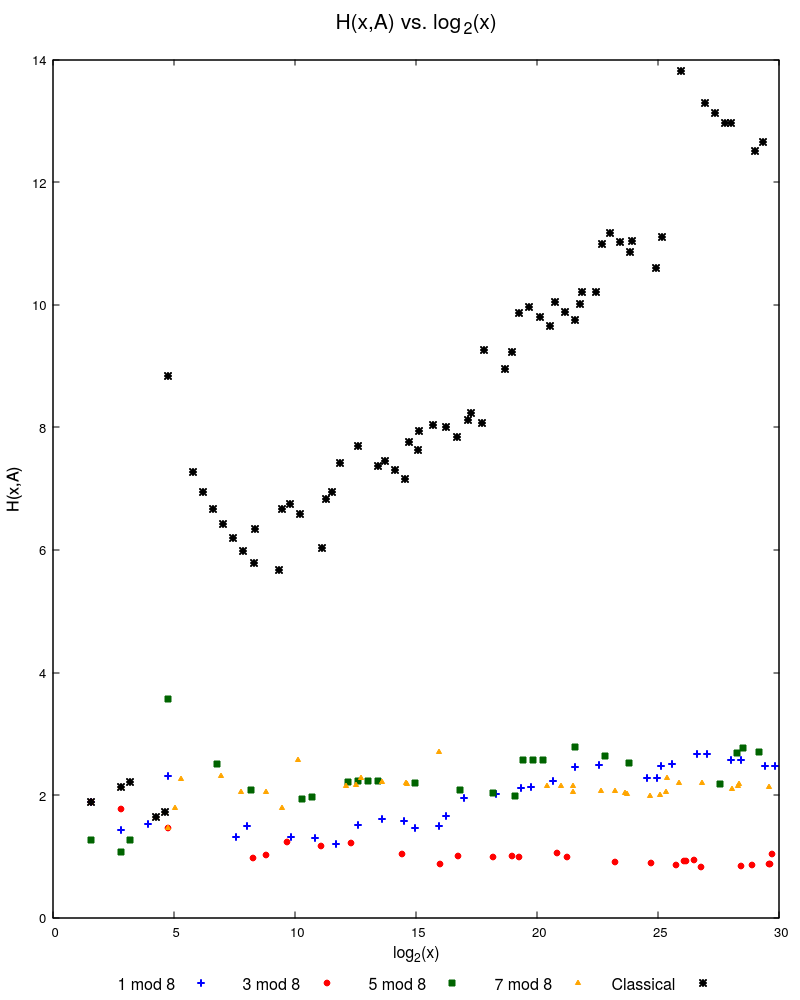
\includegraphics[scale=0.75]{ModAvoidanceAnalysisPics/H_vs_log.png}
    \caption{This graph visualizes how the $H$ values for Collatz Variants 1, 3, 5, and 7 compare to each other, and to classical hardness. The log of the record holding numbers, or number of bits needed, is the x-axis, and the hardness measure $H$ as defined in subsection~\ref{subsec:algdefinemeasure} is the y-axis.}
    \label{fig:hvslog}
\end{figure}
Comparing the three unproven Collatz Variants 1, 5, and 7 to the proven variant 3, the known variant is easier. The known variant actually slight decreases in hardness as the number of bits increases, meaning that there are fewer odd numbers per bit than the unproven variants. \par
Comparing the unknown variants to themselves, there is no consistent leader among the three as the number of bits increases. However, they all seem to be around within a hardness range of 1-3, with only a couple of exceptions. Variant 7 seems to remain in the same range with no definite increase or decrease, whereas variants 1 and 5 grow slightly from around 12 bits onward. The growth for both variants 1 and 5 may be because as numbers get larger, there are more opportunities to visit the $6 \rightarrow 7 \rightarrow 6$ cycle, which cleraly adds odd numbers more quickly to the sequence than any other base 8 graph traversal. More experiments for higher numbers should be consider in order to determine whether any of these three unknown variants trend the same way as we add more bits into the computation.
Classical Hardness actually tends to grow linearly against the log scale, meaning that as the input number increases, determining if the input number converges to 1 gets logarithimcally harder. This contrasts to all three unproven variants, which tend to stay between values of 1.5 and 3 for $H$ for numbers below 1 billion, meaning that figuring out proofs for the variants' termination is expected to be easier than proving the Collatz Conjecture.
\subsection{Percentage of Sequence Function Results and Analysis} \label{subsubsec:algsinpercentage}
 Figure~\ref{fig:pvslog} shows the results of $P(x,A)$ versus the number of bits.\par 
\begin{figure}
    \centering
    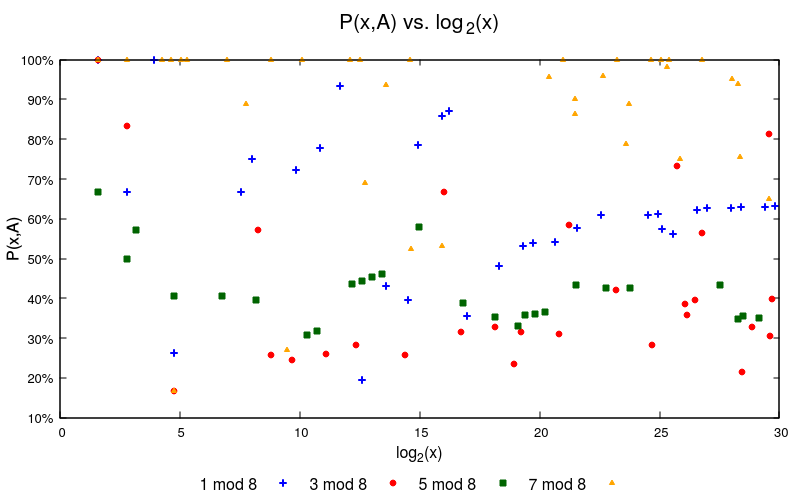
\includegraphics[scale=0.75]{ModAvoidanceAnalysisPics/P_vs_log.png}
    \caption{This graph visualizes how the $P$ values for Collatz Variants 1, 5, and 7 compare to each other. The log of the record holding numbers, or number of bits needed, is the x-axis, and the percentage measure $P$ as defined in subsection~\ref{subsec:algdefinemeasure} is the y-axis.}
    \label{fig:pvslog}
\end{figure}

$P(x,A)$, as discussed earlier, is just calculating what percentage of the record sequence contributes to the overall decay of that sequence to 1. \par
Collatz Variant 7 comprises the highest percentage overall, with a couple of exceptions. Following Collatz Variant 7 causes the sequence to decline rapidly, since the $6 \rightarrow 7 \rightarrow 6$ cycle causes an input number to grow faster than any other cycle in the base 8 graph. Almost all of the records for variant 7 terminate at 1 instead of actually reaching a number that is $7 \Mod{8}$. \par
Variant 5 tends to have a low percentage, and is the least erratic of all four variants, meaning the standard deviation is lower. Variant 5 avoids the 0 self-cycle, which causes many divisions by 2. Numbers having a long sequence that prevent termination of variant 5 tend to have a very large number when they finally reach a number that is $5 \Mod{8}$, meaning that often, many more steps in the $3x+1$ mapping must be taken before these numbers converge to 1. \par
Variant 1 is interesting, because as the input numbers grow larger, the line changes from erratic behavior to a more steady percentage between approximately 50\% and 60\% at around 20 bits. This is likely a consequence of the sequence similarity that is seen in larger record for variant 1, which will be analyzed in subsubsection~\ref{subsubsec:algseqsim}. Further, as mentioned in the cycle analysis for the $4 \rightarrow 6 \rightarrow 3 \rightarrow 2 \rightarrow 5 \rightarrow 0 \rightarrow 4$ cycle (allowing $6 \rightarrow 7 \rightarrow 6$, but avoiding 1), avoiding $1\Mod{8}$ causes a clash between the decay of the 0 self-cycle and the growth of the $6 \rightarrow 7 \rightarrow 6$ cycle, which may explain some of the erratic behavior for variant 1, aside from the small part with chain similarity.
Variant 3 tends toward the lowest percentage of all odd numbers, even lower than variant 5, but also has erratic behavior. This could be explained by the fact that avoiding termination of variant 3 causes the sequence to follow some combination of the $6 \rightarrow 7 \rightarrow 6$ cycle, the $4 \rightarrow 2 \rightarrow 1 \rightarrow 4$ cycle, or the $4 \rightarrow 2 \rightarrow 5 \rightarrow 0 \rightarrow 4$ cycle with some number of $0$ self-cycles. The first cycle causes growth, whereas all three other cycles cause decay. If the growth cycle is followed, the number gets larger, likely reducing the percentage of odd numbers making up long chains avoiding termination of variant 3, whereas the decay cycles cause the number to shrink, tending the percentages to be higher. This may explain why variant 3 causes widely different percentages.
\subsection{Sequence similarity analysis} \label{subsubsec:algseqsim}
We analyzed the sequences of the records for Collatz Variants 1, 5, and 7 as well to see if we could find any similarities:
\begin{itemize}
    \item Variant 1: There are two groups of records that were particularly interesting: Those from 325,791 to 32,505,681 (call this group $S$), and those from 35,651,835 to 949,643,331 (call this group $T$). Group $S$ numbers all terminated at number 161, and group $T$ numbers all terminated at number 35,369. These sequences all matched \textit{number-by-number} at least one other sequence starting at most 8 steps from the beginning. This is a striking similarity meaning that records for variant 1 might be predictably related to groups $S$ or $T$, or perhaps to other groups.
    \item Variant 7: All record sequences, except for input number 27, terminated at 1. While there was some similarity between sequences (all numbers $\geq 62079$ had the same last 41 numbers), there were many different paths taken from the input, so not as many patterns here.
    \item Variant 5: This had few matches and was the most changing of the records, so chain similarity appears not to have did not have as much to do with the low standard deviation for $P$ we saw for variant 5. 
\end{itemize}
\section{Paired Base Avoidance Analysis} \label{subsec:algpairedbase}
Because it appears to be difficult to figure out why Collatz Variants 1, 5, and 7 must terminate, we also analyzed the unknown variant $\{5,7\}$. This section will analyze what happens to $H(x,A)$ and $P(x,A)$ where $A$ is equal to three different base sets: the unknown variant $A=\{5,7\}$, and the known variants where $A=\{1,5\}$, and $A=\{1,7\}$. The known variant $\{1, 5\}$ has not been proven yet but a quick proof is shown here:
\begin{lemma}
The Collatz Variant $\{1, 5\}$ must terminate.
\end{lemma}
\begin{proof}
We already know that Collatz Variant 2 must terminate. Looking at the base 8 graph, 2 must traverse to either node 1 or 5. Clearly, variant $\{1, 5\}$ must terminate for any $N$.
\end{proof}
The termination of variant $\{1, 7\}$ was discussed in~\ref{subsubsec:cycleanalysis}. We decide to include both variants to compare it to variant $\{5, 7\}$.
\subsection{Hardness Function Results and Analysis} \label{subsubsec:algmulhardness}
Figure~\ref{fig:h_multivslog} shows the results of $H(x,A)$ versus $\log_2{x}$. Total steps for each mod number were also added in as well.\par
\begin{figure}
    \centering
    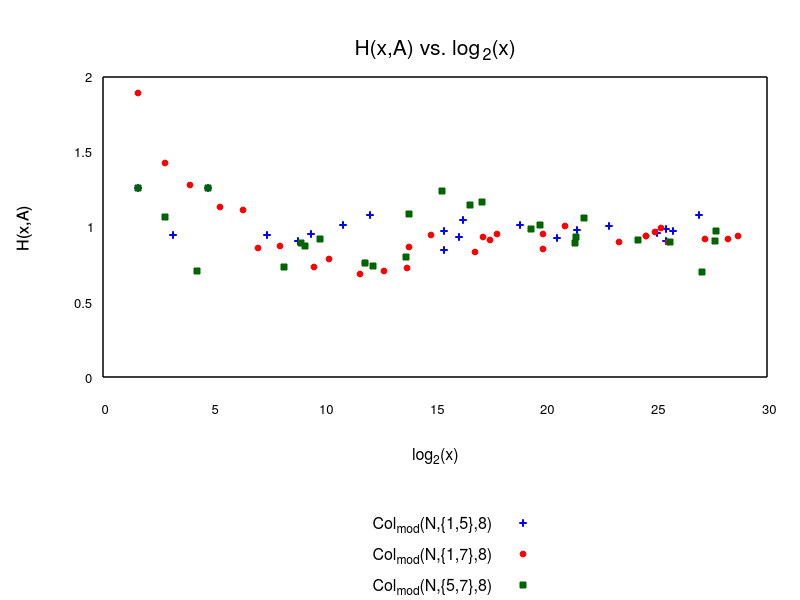
\includegraphics[scale=0.75]{ModAvoidanceAnalysisPics/H_vs_log_multi_base.png}
    \caption{This graph visualizes the $H$ measure for the three Collatz Variants $\{1,5\}$, $\{1,7\}$, and $\{5,7\}$. The log of the record holding numbers, or number of bits needed, is the x-axis, and the hardness measure $H$ as defined in subsection~\ref{subsec:algdefinemeasure} is the y-axis. Classical Hardness was omitted from this graph to eliminate distortion.}
    \label{fig:h_multivslog}
\end{figure}
These results were quite surprising. At first thought, it would have appeared that the unproven variant $\{5, 7\}$ should be the hardest to determine, compared to the two variants we have proofs for. But both variants $\{1, 5\}$ and $\{1, 7\}$  had alike predictive hardness to $\{5, 7\}$! These numbers suggest that a proof for determining why variant $\{5, 7\}$ must terminate is either easier than we anticipated, or our hardness measures are not very good. However, given the fact that variant 3 for the single base cases is clearly easier than variants 1, 5, and 7, we have reason to believe this measure should be good. Further investigation needs to be considered.
\subsection{Percentage of Sequence Function Results and Analysis} \label{subsubsec:algmulpercentage}
Figure~\ref{fig:p_multi_vslog} shows the results of $P(x,A)$ versus $\log_2{x}$.\par
\begin{figure}
    \centering
    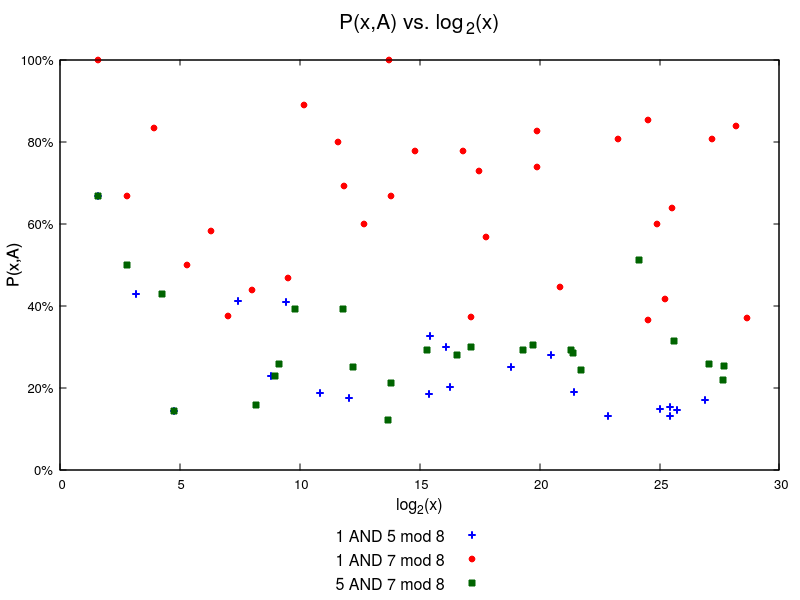
\includegraphics[scale=0.75]{ModAvoidanceAnalysisPics/P_vs_log_multi_base.png}
    \caption{This graph visualizes the $P$ measure for variants $\{1,5\}$, $\{1,7\}$, and $\{5,7\}$. The log of the record holding numbers, or number of bits needed, is the x-axis, and the hardness measure $P$ as defined in subsection~\ref{subsec:algdefinemeasure} is the y-axis.}
    \label{fig:p_multi_vslog}
\end{figure}
The variant $\{1,7\}$ makes up the highest percentage of the sequence compared to the other two cases, because avoiding both the $6 \rightarrow 7 \rightarrow 6$ and the $4 \rightarrow 6 \rightarrow 3 \rightarrow 2 \rightarrow 1$ cycles only allows for the sequence to go through the $4  \rightarrow 2 \rightarrow 5 \rightarrow 0 \rightarrow \ldots \rightarrow 4$ cycle, causing fast decay, like with variant 7. \par
Both variants $\{1,5\}$ and $\{5,7\}$ are much closer to each other in percentage of total sequence, although as the numbers grow past 17 bits in size, variant $\{5,7\}$ comprises of the higher percentage of the sequence. A possible explanation is the fact that the $6 \rightarrow 7 \rightarrow 6$ cycle allowed in variant $\{1,5\}$ allows causes a number to grow larger than the $4 \rightarrow 6 \rightarrow 3 \rightarrow 2 \rightarrow 1$ cycle that variant $\{5,7\}$ allows, and since variant $\{1,5\}$ allows for larger numbers, and the fact that larger numbers generally (but not always) take more steps to decline, that allowing for more growth should mean that the long sequence avoiding termination of variant $\{1,5\}$ should make up a lower percentage of all odd numbers.


%MENTION SAT SOLVERS VERY BRIEFLY HERE.

\chapter{Using SAT Solvers with String Rewriting Systems} \label{sec:SRSandSAT}
In this chapter, we talk briefly about SAT solvers, string rewrite systems, how we can use SAT solving to determine if a string rewrite systems terminates for any input, and a string rewrite system that Aaronson built, which, if this system terminates, we believe it is equivalent to showing that the Collatz Conjecture holds. We then present results of an attempt that Heule built using Aaronson's rewrite system.
\section{SAT Solvers}
SAT solvers are powerful devices that can solve some incredibly complex problems, such as those found in hardware verification, software verification, and combinatorics. SAT solvers leverage the fact that $k$-SAT, where $k$ is the maximum number of literals per clause, is a decision problem derived from SAT that is NP-Complete when $k > 2$, meaning that if $P \ne NP$, the worst case runtime is exponential. However, with clever heuristics, we can actually make any propositional logic formulas run in linear time for many interesting cases. Knowing SAT solving background is not important for this Thesis, but there is a great deal of literature talking about SAT solving background, so one can check, for instance,~\cite{Biere:2009:HSV:1550723}.
\section{String Rewrite Systems}
A string rewriting system (SRS), at a high level, takes a input string of an alphabet, and applies string rewriting rules (SRRs) in an arbitrary order on the input string to see if the string can be transformed further.  An example SRS is given.
\begin{definition}{SRS A:} 
The alphabet is $\Sigma = \{a, b, c\}$ and the SRRs are as follows:
\begin{enumerate}
    \item $aa \rightarrow bc$
    \item $bb \rightarrow ac$
    \item $cc \rightarrow ab$
\end{enumerate}
\end{definition}
A problem, called Zantema's Other Problem~\cite{Hofbauer:2006:TA:1142725.1711178}, using SRS A, asks the following question:\par\noindent
\begin{question}{Zantema's Other Problem:}
Does the system laid out in SRS $A$ terminate for any input string $(a|b|c)*$?
\end{question}
If one thinks about this problem a little, it would seem that a proof to show that this problem terminates for all input strings should be easy to show.  Surprisingly, both humans and computers struggled to come up with a proof for this problem when initially presented.  However, Hofbuaer and Waldmann came up with a proof for determining that it terminates~\cite{Hofbauer:2006:TA:1142725.1711178}, and from this, found that, for any rewriting rules in any rewrite system, if they are transformed into functions that causes all inputs to decrease, then the rewrite system will terminate.~\cite{Hofbauer2006}. \par
The matrices are built using SAT solving to determine if a $d \times d$ matrix is large enough to ensure that the matrix functions for the set of rewrite rules always decrease for all inputs. The process of building these matrices is described in a paper by Endrullis, Waldmann and Zantema~\cite{Endrullis2006}. An example using Zantema's Other Problem will be explained here.\par
Here are the matrices computed by SAT from ~\cite{Hofbauer:2006:TA:1142725.1711178}:
%FIX THIS OVERFULL PROBLEM HERE AND IN THE NEXT SET.
\[
a(\Vec{x}) = \begin{pmatrix}
1&0&0&3\\
0&0&2&1\\
0&1&0&1\\
0&0&0&0
\end{pmatrix} \Vec{x} + \begin{pmatrix}
1\\
0\\
1\\
0
\end{pmatrix}
b(\Vec{x}) = \begin{pmatrix}
1&2&0&0\\
0&2&0&1\\
0&1&0&0\\
0&0&0&0
\end{pmatrix} \Vec{x} + \begin{pmatrix}
1\\
2\\
0\\
0
\end{pmatrix}
c(\Vec{x}) = \begin{pmatrix}
1&0&0&1\\
0&0&0&1\\
0&1&0&1\\
0&2&0&0
\end{pmatrix} \Vec{x} + \begin{pmatrix}
1\\
0\\
3\\
0
\end{pmatrix}
\]
We will show an example string to show that it is always decreasing, but first, define the $\succ$ operator to show that, for vectors $(x_1 \ldots x_d)$ and $(y_1 \ldots y_d)$, $(x_1 \ldots x_d) \succ (y_1 \ldots y_d)$ if $x_1 > y_1$ and $x_i \geq y_i$ for $i \in \{2, \ldots, d\}$. In other words, the first element of a vector must be always decreasing, while the other $d-1$ elements must either be the same or decrease. \par
Let our sample string be $bbaa$. Here is a possible set of rules that can be applied to it as well as the vector representations of the symbols:
%FIX THIS OVERFULL PROBLEM HERE
\begin{align*}
    bb\underline{aa} &\rightarrow b\underline{bb}c &\rightarrow ba\underline{cc} &\rightarrow b\underline{aa}b &\rightarrow \underline{bb}cb &\rightarrow a\underline{cc}b &\rightarrow aa\underline{bb} &\rightarrow a\underline{aa}c &\rightarrow ab\underline{cc} &\rightarrow abab \\
    \begin{pmatrix}18\\14\\6\\0\end{pmatrix} &\succ
    \begin{pmatrix}17\\14\\6\\0\end{pmatrix} &\succ
    \begin{pmatrix}15\\14\\6\\0\end{pmatrix} &\succ
    \begin{pmatrix}14\\14\\6\\0\end{pmatrix} &\succ
    \begin{pmatrix}13\\14\\6\\0\end{pmatrix} &\succ
    \begin{pmatrix}7\\14\\5\\0\end{pmatrix} &\succ
    \begin{pmatrix}6\\14\\5\\0\end{pmatrix} &\succ
    \begin{pmatrix}4\\14\\3\\0\end{pmatrix} &\succ
    \begin{pmatrix}3\\0\\3\\0\end{pmatrix} &\succ
    \begin{pmatrix}2\\0\\3\\0\end{pmatrix}
\end{align*}
The vector representation of the strings are always decreasing as defined by the $\succ$ operator. We could apply any string with symbols $a$, $b$, and $c$ and apply rules until termination and the vectors representing the strings would always decrease.
\section{The Collatz Conjecture as a rewriting system} \label{subsec:CollatzSRS}
Aaronson built an SRS representing the Collatz Conjecture~\cite{HeuleAaronson}. We'll call this the Collatz SRS throughout the remainder of this Thesis. \par
Let the alphabet of the Collatz SRS consist of the symbols $a, b, c, d, e, f, g$. The symbols can be written as these linear functions:
\[
a(x) = 2x, b(x) = 2x+1, c(x) = 1, d(x) = x, e(x) = 3x, f(x) = 3x+1, g(x) = 3x+2
\]
%the binary symbols and ternary symbols part is a bit awkward, but decided to come back to it later.
The symbols $a$ and $b$ are binary symbols. They represent  a binary system: $a$ is 0 and $b$ is 1.  The symbols $e$, $f$, and $g$ are ternary symbols. They represent a ternary system: $e$ is 0, $f$ is 1, and $g$ is 2. $c$ and $d$ are placeholder symbols to represent the leading 1 and the end of the string, respectively. They help this rewrite system know where the beginning and end of the string are. \par
Note that in order to correctly compute the values that the strings represent using the above linear functions, one needs to read the functions from left to right. That is to say, the string $cabad$, which is equal to 10, is not equal to $ c \circ a \circ b \circ a \circ d$, where $\circ$ is the composition of functions. Instead, $cabad = d \circ a \circ b \circ a \circ c$. Aaronson chose to write the strings like this since they follow the way we would write numbers. \par
Using the provided alphabet, Aaronson created the following series of SRRs:
\begin{align*}
    D_1 : ad &\rightarrow d\ & \ A_1 : ae &\rightarrow ea\ & \ B_1 : be &\rightarrow fb\ & \ C_1 : ce &\rightarrow cb \\
    D_2 : bd &\rightarrow gd\ & \ A_2 : af &\rightarrow eb\ & \ B_2 : bf &\rightarrow ga\ & \ C_2 : cf &\rightarrow caa \\
    &\ &\ A_3 : ag &\rightarrow fa\ &\ B_3 : bg &\rightarrow gb\ &\ C_3 : cg &\rightarrow cab
\end{align*}
The SRRs provided here allow for Aaronson's SRS to be equivalent to the $3x+1$ mapping, but a formal proof showing this is the case is difficult, because we have yet to find a proof showing that the rewrite rules can be applied in arbitrary order. However, we can explain how the rules work, and show that any valid input string correctly follows the $3x+1$ mapping for the number the string represents, and after this, we will show the ordering we follow, and why this ordering is correct. \par
Each of the rules denotes how to handle the symbols $a-g$, or the combination of binary and placeholder strings. The $D$ rules represent the two steps taken by the Collatz Conjecture in a binary system. $D_1$ is how we handle an even number. It computes division of $x$ by 2 by removing the $a$ symbol that represents a binary 0. $D_2$ is actually a combination of several steps. If we were to represent $3x+1$, we could just write $bd \rightarrow bfd$, meaning take all previous symbols and multiply the result by 3 and add 1. The problem with this rule is that it increases the size of the resulting string, making the system more difficult to prove. However, $bfd \rightarrow gad$ is a valid rule,  as $d \circ f \circ b = 3(2x+1)+1 = 6x+4$ and $d \circ a \circ g = 2(3x+2) = 6x+4$, and from here, we can apply the rule $ad \rightarrow d$ to allow us to do $gad \rightarrow gd$. Since $3x+1$ always results in an even number, we can just make rule $D_2$ compute $(3x+1)/2$ without growing the string size, ultimately making rule $D_2$ into $bd \rightarrow gd$. $D_2$ is the rule that makes termination of our system hard to prove. Without it, we would not need the $A$, $B$, or $C$ rules.\par
The $A$, $B$ and $C$ rules all deal with the handling of the ternary symbols and the eventual conversion of these ternary symbols into the binary symbols. The $A$ and $B$ rules deal with the case when a ternary symbol is to the right of the binary symbol, and how to switch the ternary symbol and the binary symbol without changing the number the string represents. We will show that all 6 of these rules preserve the same number by showing that the string represents the same value after each rule has been applied:
\begin{itemize}
    \item $\boldsymbol{ae \rightarrow ea}$: $ae = e \circ a = e(a(x)) = 2(3x) = 6x$, and $ea = a
    \circ e = a(e(x)) = 3(2x) = 6x$.
    \item $\boldsymbol{af \rightarrow eb}$: $af = f \circ a = f(a(x)) = 3(2x)+1 = 6x+1$, and $eb =
    b \circ e = b(e(x)) = 2(3x)+1 = 6x+1$.
    \item $\boldsymbol{ag \rightarrow fa}$: $ag = g \circ a = g(a(x)) = 3(2x)+2 = 6x+2$, and $fa = a \circ f = a(f(x)) = 2(3x+1) = 6x+2$.
    \item $\boldsymbol{be \rightarrow fb}$: $be = e \circ b = e(b(x)) = 3(2x+1) = 6x+3$, and $fb = b \circ f = b(f(x)) = 2(3x+1)+1 = 6x+3$.
    \item $\boldsymbol{bf \rightarrow ga}$: $bf = f \circ b = f(b(x)) = 3(2x+1)+1 = 6x+4$, and $ga =  a \circ g = a(g(x)) = 2(3x+2) = 6x+4$.
    \item $\boldsymbol{bg \rightarrow gb}$: $bg = g \circ b = g(b(x)) = 3(2x+1)+2 = 6x+5$, and $gb = b \circ g = b(g(x)) = 2(3x+2)+1 = 6x+5$.
\end{itemize}
Hence, these rules are all correct. \par
The $C$ rules take advantage of the fact that the $c$ symbol is a binary 1, and, in a strictly binary string, it is the most significant bit of the corresponding number $x$. When the ternary symbol is adjacent to the $c$ symbol, we apply one of the three $c$ rules to convert the ternary symbol into binary symbol(s). These rules also preserve the number the string represents, and the proofs showing this is the case for each of these rules are shown here:
\begin{itemize}
    \item $\boldsymbol{ce \rightarrow cb}$: $ce = e \circ c = e(c(x)) = 3(1) = 3$, and $cb = b
    \circ c = b(c(x)) = 2(1)+1 = 3$.
    \item $\boldsymbol{cf \rightarrow caa}$: $cf = f \circ c = f(c) = 3(1)+ 1 = 4$, and $caa = a \circ a \circ c = a(a(c(x))) = 2(2(1)) = 4$.
    \item $\boldsymbol{cg \rightarrow cab}$: $cg = g \circ c = g(c) = 3(1)+ 2 = 5$, and $cab = b \circ a \circ c = b(a(c(x))) = 2(2(1))+1 = 5$.
\end{itemize}
Hence, we have shown that the $A$, $B$, and $C$ rules all preserve value, and the $D$ rules correctly apply the $3x+1$ mapping. \par
Here is how one can run the SRS and preserve an ordering we know to be valid:
\begin{enumerate}
    \item Take the initial input number, and convert it to binary. Make the leading 1 a $c$ symbol, and all 0's and other 1's $a$'s and $b$'s, respectively.
    \item Until we have the string $cd$: 
    \begin{itemize}
        \item Apply the appropriate $D$ rule.
        \item If $D_2$ is applied, apply $A$ and $B$ rules until the ternary symbol and the $c$ are adjacent, then apply the appropriate $C$ rule.
    \end{itemize}
\end{enumerate}
This order of applying the SRRs is correct, because one takes a string that is strictly in binary symbols and applies the correct $D$ rules until rule $D_2$ is applied, then it handles the ternary symbol immediately by applying $A$, $B$, and $C$ rules until it is converted into binary symbol(s). The number is not changed during application of these rules, making the ordering correct. This ordering was used in building the system that investigated the number of steps needed in the rewrite system, which will be talked about in section~\ref{sec:hardnessrewriterules}. \par
If we take this SRS and model matrix functions for all symbols that cause all inputs to decrease, then we believe we can prove the Collatz Conjecture. We don't have an absolute link, but we strongly believe that termination of the Collatz SRS implies termination of Algorithm~\ref{alg:ColR}, since the rewrite system operates on input strings the same way as would Algorithm~\ref{alg:ColR} operate on positive integers.
\section{Proving Collatz Conjecture Results} \label{subsec:provingCollatzresults}
This section discusses some of the results mentioned in~\cite{HeuleAaronson}. Heule and Aaronson have not been able to prove termination of the Collatz SRS for all 11 rules, which is why this investigation for Collatz subproblems came about. This section describes the results thus far. \par
Heule tried to run the Collatz SRS on state-of-the-art matrix interpretation solvers like AProVE. However, 4 of the 11 rules needed to be removed before the system could be solved. So a custom matrix interpretation solver was built by Heule specifically for this problem. 
Unfortunately, Heule could not prove the entire 11 rule system with matrix interpretation. However, any combination of 10 of the 11 rules can be proven. Some were very easy (example: omitting rule $D_2$), others much more challenging.\par
Hence, the motivation for simplifying the problem by creating the Collatz Variants derived from~\ref{alg:ColSP}, came about, as did the motivation for writing this thesis. Chapter~\ref{sec:hardnessrewriterules} investigates alterations of the SRR's for the Collatz SRS, which we call  to try and make the problem simpler for the matrix interpretation solver, and see how difficult these alternate forms ought to be to prove.


%I need to make sure that I define subproblems clearly here to mean SRSs with rewrite rules. That's going to be a bit later.

\chapter{Hardness of Application of Rewrite Rules} \label{sec:hardnessrewriterules}
%\textbf{****NOTE! This chapter is going to be heavily rewritten for the next iteration. Feel free to look at it now if you have time, but it may be drastically different next time.****}\par
%Outline:
%-Scott mentioned that he expects the number of rewrite steps needed is O(log(N)^2), where N is the input number. My findings are consistent with this. I ran the rewrite system for all Delay Records found on Roosendaal's website up to 1 billion: http://www.ericr.nl/wondrous/delrecs.html
%        -I took steps that the rewrite system and divided by O(log(N)^2). The constant never exceeds 15.37. This is well bounded by the highest Gamma constant I found up to 1 billion: 32.89.
%        -Recall that Gamma is defined by:
%            -Steps to reach 1 = Gamma * ln(N) (From Lagrias's Survey)
%            -The max Gamma found by Eric Roosendaal is 36.72 for approximately 7.2*10^21 (source: http://www.ericr.nl/wondrous/comprecs.html)
%-Hardness of 1, 5, and 7 mod 8 from a rewrite perspective: I'll compute H_r(x,A) = # of rewrite steps we avoid A mod 8/log^2(N), and compare 1, 5, and 7 mod 8 to each other.
%        -I should also do the same with the number of rewrite steps for the normal Collatz Delay Records and compare these to 1, 5, and 7 mod 8.
% -Exploring modifications of the rewrite system:
%        -I used a modified rewrite system that Marijn told me about (eliminating the ad -> d rule) on the Delay Records from Roosendaal's website, and found that we decrease rewrite steps between around 7% - 25%. However, the larger the number, the smaller percentage the decrease.
%        -Want to present results and leave as an open suggested topic for further optimizations. I'm open to taking any other suggestions before I finish this Thesis.
Now we have explained the background for Rewrite Systems, as well as the motivation for them, we now build on top of the  algebraic hardness measure computation done in chapter~\ref{sec:subhrdnspred}. First, we discuss a program we created that replays the Collatz SRS for certain numbers, which is used throughout this chapter. Then, we attempt to establish a reasonable upper bound for number of rewrite steps needed. We then use this upper bound to compute reasonable hardness measures for modifications of the Collatz SRS that align with the earlier discussed variants. Finally, we explore another modification to Aaronson's rewrite system which reduces rewrite steps.% First, we do computations with slight modifications to the Collatz SRS, and second, we only compute record sequences from our previous algebraic analysis. In this section, we first introduce a modified version of the SRS, then we define measures, talk about the computation, then present our results.
\section{Computation} \label{subsec:rewritecomp}
The program we wrote simulates the Collatz SRS in Java. It takes two different keys of input: some positive integers (either one number, or a batch of numbers, one per line), and a string file which has one SRR per line in the format ``input output'', which is equivalent to the rule $input \rightarrow output$. The \# character is a comment, meaning if the first character of a rewrite rule is \#, we ignore that line. This is a convenience to comment out a rule to create SRRs that correspond to Collatz subproblems. The output is a file with the transformation of the rewrite terms, and which number these terms correspond to. If a batch of numbers is run, one file is made for each number. Also, an aggregate file can be printed for batches that lists the input number, the final number, and the number of rewrite steps. \par
The program converts an input number into a binary rewrite string with characters $a$, $b$, $c$, and $d$. The rewrite term is stored in an array that has a ``sliding'' string in it. This is the most efficient way to take advantage of Aaronson's SRS, because a number only grows from the $c$ term, and shrinks from the $d$ term. Hence, the spare space of the array is past the $c$ term, and any time a $D$ rule decreases size, we move in the end of the $d$ symbol, and all other symbols past it are thrown out if more space is needed. For instance, when we apply rule $D_2$, the $a$ term gets replaced with a $d$ term, and a pointer denoting the end of the string gets moved to the new $d$ symbol. If we run out of space in the array, we double the size of it, discarding any unnecessary terms past the leading $d$. \par
As discussed in section~\ref{subsec:CollatzSRS}, we don't apply SRRs in arbitrary order. Given a rewrite string completely in binary, we check to see if any $D$ rule can be applied. If not, the program terminates. If we do find a $D$ rule, then apply it, and check if a ternary character is generated by it. If so, we apply the $A$ and $B$ rules to move the ternary character index-by-index until we can apply a $C$ rule, which removes the ternary character. \par
The code can be accessed via a public GitHub repository located at \url{https://github.com/mdenend/CollatzRewriteSystem}. A readme file is included that explains how to run the code and available options.


\section{Estimated rewrite steps needed} \label{subsec:estrwsteps}
Looking at how the Collatz SRS operates, one can establish a reasonable bound on how many more steps the Collatz SRS adds compared to the algebraic method of computing Collatz Sequences. Starting with a number that is purely in binary symbols $a$ and $b$, plus the placeholder symbols $c$ and $d$, there are two different events that can occur. When $a$ is the symbol to the immediate left of the $d$, we divide by 2. It only takes one step to complete this division. On the other hand, when we compute an odd number, we turn the $b$ symbol into a $g$ symbol, and, following the establised order, apply $A$, $B$, and $C$ rules to conver the ternary symbol to binary. This adds $\Theta(m)$ rewrite steps per odd number. \par
We can compare the number of steps that the rewrite system takes to Classical Hardness records from chapter~\ref{sec:subhrdnspred}. If we do in fact apply a factor of $\Theta(m)$ more steps per odd number in our rewrite system, then Classical Hardness should be pretty close to $\frac{\text{Rewrite Steps for Odd Numbers}}{\log^2{m}}$ for Classical Hardness records input into the Collatz SRS. The results of this analysis are presented in Figure~\ref{fig:rvc_log}. From this graph, it appears that dividing the odd number of rewrite steps by $\log{m}$ creates a reasonably tight bound against Classical Hardness, so given the numbers we measures, the Collatz SRS adding a factor or $\Theta(m)$ rewrite steps per odd number appears to be correct.
\begin{figure}
    \centering
    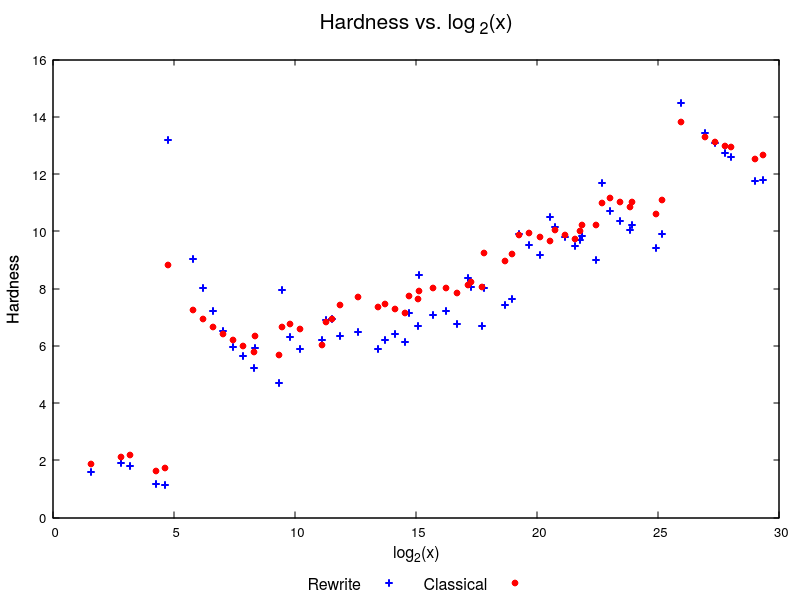
\includegraphics[scale=0.75]{ModAvoidanceAnalysisPics/RvC_vs_log.png}
    \caption{This graph compares, on the same set of input numbers, Classical Hardness as defined in chapter~\ref{sec:subhrdnspred}, and Rewrite Hardness, which is the number of steps divided by the number of input bits squared. The log of the record holding numbers, or number of bits needed, is the x-axis, and the hardness is the y-axis.}
    \label{fig:rvc_log}
\end{figure}


\section{Collatz SRS Subproblem Analysis} \label{subsec:collatzsubproblemananalysis}
Although it appears that the rewrite system adds a factor of $\log{m}$ steps to solving the Collatz Conjecture, this does not mean that the hardness of the Collatz Variants will not differentiate, given the fact that certain variants may deal with different sized numbers. This section takes the Collatz SRS and modifies it so it can compute Algorithm~\ref{alg:ColSP}, but with strings instead of numbers.
\subsection{Modified Base 8 Rewrite System} \label{subsec:base8rewrite}
Now we have established a reasonable bound of how many more steps the rewrite system adds, let us explore how we can modify the Collatz SRS to make it tie into our variants. Recall the $D$ rules of the Collatz SRS: the rules that handle the even and odd numbers:
\begin{align*}
    D_1: ad &\rightarrow d &\text{$0\Mod{2}$}\\
    D_2: bd &\rightarrow gd &\text{$1\Mod{2}$}\\
\end{align*}
$D_1$ handles $0 \Mod{2}$ (even numbers) by effectively dividing by 2, while $D_2$ handles $1 \Mod{2}$ (odd numbers)  by effectively computing $3x+1/2$. Also note that all input strings for these rules are just one bit, since the placeholder $d$ is not a digit. However, we can expand this input to be 3 bits and come up with 8 corresponding SRRs:
\begin{align*}
    aaad &\rightarrow aad &\text{$0\Mod{8}$}\\
    aabd &\rightarrow ebad &\text{$1\Mod{8}$}\\
    abad &\rightarrow abd &\text{$2\Mod{8}$}\\
    abbd &\rightarrow fabd &\text{$3\Mod{8}$}\\
    baad &\rightarrow bad &\text{$4\Mod{8}$}\\
    babd &\rightarrow gaad &\text{$5\Mod{8}$}\\
    bbad &\rightarrow bbd &\text{$6\Mod{8}$}\\
    bbbd &\rightarrow gbbd &\text{$7\Mod{8}$}
\end{align*}
It is easy to see how these rules all correspond to a node in graph $G_8$: an input string strictly with symbols $a$, $b$, $c$, and $d$ corresponds to a binary number. The inputs, in order, are numbers congruent moduly to 0-7$\Mod{8}$, and the outputs are the result of dividing by 2, if even, or multiplying by 3 and adding 1. All of the odd rules, like rule $D_2$ in the original system, are just a combination of several rules, which ensure that the output string is not longer, and it reduces a couple of steps by moving the ternary term toward the front. All of the even number node rules are just the same exact rule $D_1$ in the original system, so we can remove any even rules and replace them with the original $D_1$. Hence, we use the following SRRs in the base 8 modification of the Collatz SRS:
\begin{align*}
    D_{8_1}: ad &\rightarrow d &\text{$0\Mod{2}$}\\
    D_{8_2}: aabd &\rightarrow ebd &\text{$1\Mod{8}$}\\
    D_{8_3}: abbd &\rightarrow fabd &\text{$3\Mod{8}$}\\
    D_{8_4}: babd &\rightarrow gd &\text{$5\Mod{8}$}\\
    D_{8_5}: bbbd &\rightarrow gbbd &\text{$7\Mod{8}$}
\end{align*}
Because these rules were constructed using only SRRs in the Collatz SRS that we know to be correct, we know these new $D$ rules, plus the $A$, $B$, and $C$ rules, are equal to the original Collatz SRS. However, they do add an extra dimension not present before. We can remove one of the rules to make it easier to prove that the derived SRS will terminate. We present a sample SRS with rule $D_{8_2}$ removed:
\begin{align*}
    D_{8_1}: ad &\rightarrow d &\text{$0\Mod{2}$}\\
    D_{8_3}: abbd &\rightarrow fbbd &\text{$3\Mod{8}$}\\
    D_{8_4}: babd &\rightarrow gd &\text{$5\Mod{8}$}\\
    D_{8_5}: bbbd &\rightarrow gbbd &\text{$7\Mod{8}$}
\end{align*}
Since we removed the SRR that corresponds to input $1 \Mod{8}$, termination of this SRS implies termination of Collatz Variant 1, as removing a rule causes any string with this input to terminate the system. Note how removing an SRR is equivalent to adding the corresponding termination condition in Algorithm~\ref{alg:ColSP}. We call these modifications Collatz Subproblems through the rest of this section, and analyze Collatz Subproblems that would imply termination of unproven Collatz Variants.\par
\subsection{Defining Measures for Subproblem Analysis} \label{subsec:rewritemeasuredefs}
Instead of defining hardness by number of odd numbers, for the SRS, we define hardness based off of the total steps applied, because of the fact that odd numbers add significantly more steps. Define the following numbers, given some input number $x$:
\begin{itemize}
    \item $f_r(x)$: The total number of rewrite steps in the sequence for $x$ before it converges to 1.
    \item $A$: The base avoidance set, same as used in Algorithm~\ref{Col:SP} and chapter~\ref{sec:subhrdnspred}. As before, $A \subseteq \{1, 5, 7\}$ and $A \ne \varnothing$. 
    \item Collatz Subproblem $A$: Defined much in the same way as Collatz Variant $A$, but with SRS instead. Let $A$ be the same base avoidance set as in $\ColMod{N}{A}{b}$. For singleton sets $A$, we just write the number. Collatz Subprolem $A$ denotes which rewrite rule(s) are dropped, and that subproblem $A$ would imply termination of Collatz Variant $A$.
    \item Record Sequence for Collatz Subproblem $A$: Same exact definition as in chapter~\ref{sec:subhrdnspred}. We only run rewrite systems for the record sequences we computed with the algebraic Collatz program defined in subsection~\ref{subsec:algcomp}, as running computation for strictly the rewrite system would take an extremely long time.
    \item $R(x_i, A, b):$ The number of rewrite steps that the record sequence from Collatz Variant $\ColMod{x}{A}{b}$ takes in an SRS based off of Collatz Subproblem $A$. However, one big difference with $R$ is that we start at the sequence number $x_i$ such that index $i$ starts at the first number of the record sequence. This is necessary in order to correctly run the Collatz SRS for these various subproblems, because otherwise the Collatz SRS will terminate too early.
\end{itemize}
We define a hardness measure: $H_{SRS}$, where $H_{SRS} = \frac{R(x_i, A, b)}{\log_2^2{x}}$. This effectively computes the hardness of the SRRs that corresponds to determining termination of Collatz Variant $A$, but also takes into account the extra $m$ bits that the Collatz SRS adds. The number of bits we divide by is determined by our starting number, like for the analysis of Collatz Variants.

\subsection{SRR removal analysis} \label{subsec:rewritehardness}
Figure~\ref{fig:rvslog} shows the anaylsis of hardness for the modified SRS with four different Collatz Subproblems: 1, 5, 7, and $\{5,7\}$. 
\begin{figure}
    \centering
    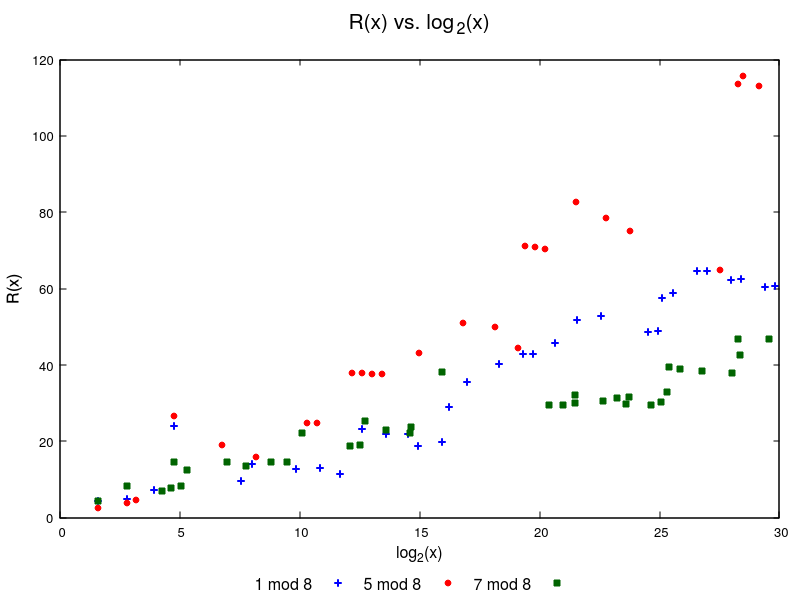
\includegraphics[scale=0.75]{ModAvoidanceAnalysisPics/R_vs_log.png}
    \caption{This graph visualizes how the $R$ values for subproblems 1, 5, and 7 compare to each other. The log of the record holding numbers, or number of bits needed, is the x-axis, and the hardness measure $R$ as defined in section~\ref{subsec:rewritemeasuredefs} is the y-axis.}
    \label{fig:rvslog}
\end{figure}
Unlike the analysis for the Collatz Variants, we have clearer separation. Subproblem 5 is the highest on almost all of its record cases. Since Collatz Variant 5 record sequences tend to grow to very large numbers, these extra bits that the large numbers generate add difficulty for the rewrite system. Further, subproblem 5 appears to get harder as the number of bits increases. Subproblem 1 exhibits the growth as numbers get bigger, but tapers off once again for numbers more than 20 bits, much like Collatz Variant 1. Subproblem 7 shows no increase as bits get larger. This suggests subproblem 7 might be easier to solve than subproblems 1 or 5. Subproblem $\{5,7\}$ has the lowest hardness, no surprise given that it has one less rule than any of the other three subproblems.
\section{Further SRS rule modifications}\label{subsec:srsrulemod}
It is possible that the set of SRRs in the Collatz SRS can be further optimized, possibly in order to solve some of the subproblems listed in this Chapter. We present one modification of the Collatz SRS by replacing the even rule with odd rules, and look at the results of doing so.
\subsection{Removing even rule from the Collatz SRS}\label{subsubsec:evenruleremove}
It is possible to replace both $D_1$ and $D_2$ in the Collatz SRS with the following set of rules that calculates with strictly odd numbers:
\begin{align*}
    D_{o1}: bbd &\rightarrow gbd &\text{$3\Mod{4}$}\\
    D_{o2}: aabd &\rightarrow ebd &\text{$1\Mod{8}$}\\
    D_{o3}: babd &\rightarrow bd &\text{$5\Mod{8}$}
\end{align*}
Rule $D_{o1}$ and $D_{o2}$ are both straightforward to see, given the fact that we talked about the base 8 modification of the Collatz SRS already. $D_{o1}$ just combines both rule $D_{8_3}$ and $D_{8_5}$, but removing the leading $a$ or $b$, respectively, and letting the $A$, $B$, and $C$ rules determine what ternary symbol we get. Rule $D_{o2}$ is exactly the same as rule $D_{8_2}$.\par
Rule $D_{o3}$ is not as intuitive at first glance, but we can look at rule $D_{8_4}$, which has the same input as $D_{o3}$, and see that the output is the same as the normal $D_2$ rule, so we can ``step backwards'' using rule $D_2$ to allow for us to get $bd$ as our output, and hence, have a full set of correct $D$ rules that go from odd number to odd number.\par
Observe that all of the $D_o$ rules have a left handed side and a right handed side ending with $bd$. As a consequence, we can remove the $b$ symbol in the second to last symbol for both the input string and the rules, resulting in the following SRRs:
\begin{align*}
    D_{o1^*}: bd &\rightarrow gd &\text{$3\Mod{4}$}\\
    D_{o2^*}: aad &\rightarrow ed &\text{$1\Mod{8}$}\\
    D_{o3^*}: bad &\rightarrow d &\text{$5\Mod{8}$}
\end{align*}
\subsection{Change in Rewrite Steps}
\begin{figure}
    \centering
    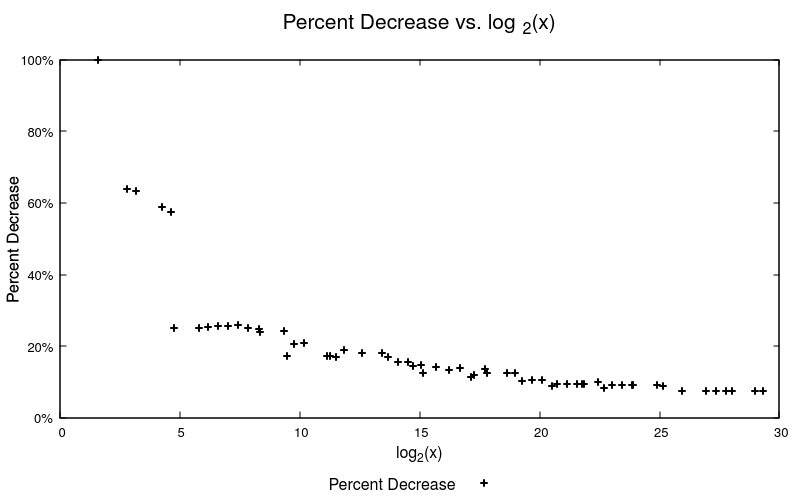
\includegraphics[scale=0.75]{ModAvoidanceAnalysisPics/Percent_Decrease.png}
    \caption{This graph shows what percentage the odd rules decrease the rewrite steps, from the original Collatz SRS. The log of the record holding numbers, or number of bits needed, is the x-axis, and the percent decrease is the y-axis.}
    \label{fig:percent_decrease}
\end{figure}
Figure~\ref{fig:percent_decrease} shows the percentage decrease for Classical Hardness records. Lower numbers tend to have a larger percentage of decrease, but as the numbers get larger, the percentage decreases. This is probably because records for larger numbers tend to have more odd numbers, meaning many more rewrite steps than lower numbers. \par
This said, the modification to the rewrite system does overall reduce the number of steps. Other SRR modifications for the Collatz SRS should be considered, as the right set of clever rules may prove termination of Collatz Subproblems, and perhaps, even proof that the Collatz Conjecture terminates.


\chapter{Conclusion} \label{sec:conclusion}
In this thesis, we analyzed the Collatz Conjecture and simpler, yet still challenging variants, and propose a hardness prediction for determining the answers to these variants. We started by building a program that investigates Collatz Variants by running many $3x+1$ sequences for all odd numbers up to 1 billion, and seeing how many odd numbers occur in record breaking sequences that avoid terminating the Collatz Variants. \par
We also investigated the Collatz SRS that Aaronson created and that Heule tried to prove with matrix interpretation. Even though this methodology has been unable to solve the Collatz Conjecture so far, we think it still has promise. We also built a simple program that ran the Collatz SRS and determined the hardness for subproblems, finding out that the hardness varies more than in the algebraic case.\par
As described in ~\cite{HeuleAaronson}, we believe this approach for trying to solve the Collatz Conjecture, as well as Collatz Variants, has merit and needs further investigation. We plan to do so under the recently approved grant.




%%%%%%%%%%%%%%%%%%%%%%%%%%%%%%%%%%%%%%%%%%%%%%%%%%%%%%%%%%%%%%%%%%%%%%
% Appendix/Appendices                                                %
%%%%%%%%%%%%%%%%%%%%%%%%%%%%%%%%%%%%%%%%%%%%%%%%%%%%%%%%%%%%%%%%%%%%%%
%
% If you have only one appendix, use the command \appendix instead
% of \appendices.
% I MAY have an appendix later on with results.
%\appendices
%\index{Appendices@\emph{Appendices}}%

%\chapter{Lerma's Appendix}
\index{Appendix!Lerma's Appendix@\emph{Lerma's Appendix}}%
The source \LaTeX{} file for this document is no longer quoted in
its entirety in the output document. A \LaTeX{} file can 
include its own source by using the command
\cn{verbatiminput\{\cn{jobname}\}}.



%%%%%%%%%%%%%%%%%%%%%%%%%%%%%%%%%%%%%%%%%%%
\chapter{My Appendix \#2}
\index{Appendix!My Appendix \#2@\emph{My Appendix \#2}}%
\section{The First Section}
This is the first section.
This is the second appendix.

\section{The Second Section}
This is the second section of the second appendix.

\subsection{The First Subsection of the Second Section}
This is the first subsection of the second section of the second appendix.

\subsection{The Second Subsection of the Second Section}
This is the second subsection of the second section of the second appendix.

\subsubsection{The First Subsubsection of the Second Subsection of
		the Second Section}
This is the first subsubsection of the second subsection of the
second section of the second appendix.

\subsubsection{The Second Subsubsection of the Second Subsection
		of the Second Section}
This is the second subsubsection of the second subsection of the
second section of the second appendix.


%%%%%%%%%%%%%%%%%%%%%%%%%%%%%%%%%%%%%%%%%%%
\chapter{My Appendix \#3}
\index{Appendix!My Appendix \#3@\emph{My Appendix \#3}}%

\section{The First Section}
This is the first section.
This is the third appendix.

\section{The Second Section}
This is the second section of the third appendix.





%%%%%%%%%%%%%%%%%%%%%%%%%%%%%%%%%%%%%%%%%%%%%%%%%%%%%%%%%%%%%%%%%%%%%%
% Generate the bibliography.					     %
%%%%%%%%%%%%%%%%%%%%%%%%%%%%%%%%%%%%%%%%%%%%%%%%%%%%%%%%%%%%%%%%%%%%%%
%								     %
% NOTE: For master's theses and reports, NOTHING is permitted to     %
%	come between the bibliography and the vita. The command      %
%	to generate the index (if used) MUST be moved to before      %
%	this section.						     %
%								     %
\nocite{*}      % This command causes all items in the 		     %
                % bibliographic database to be added to 	     %
                % the bibliography, even if they are not 	     %
                % explicitly cited in the text. 		     %
		%						     %
\bibliographystyle{ieeetr}  % Here the bibliography 		     %
\bibliography{bibliography}        % is inserted.			     %
\index{Bibliography@\emph{Bibliography}}%			     %
%\printbibliography
%%%%%%%%%%%%%%%%%%%%%%%%%%%%%%%%%%%%%%%%%%%%%%%%%%%%%%%%%%%%%%%%%%%%%%


%%%%%%%%%%%%%%%%%%%%%%%%%%%%%%%%%%%%%%%%%%%%%%%%%%%%%%%%%%%%%%%%%%%%%%
% Generate the index.						     %
%%%%%%%%%%%%%%%%%%%%%%%%%%%%%%%%%%%%%%%%%%%%%%%%%%%%%%%%%%%%%%%%%%%%%%
%								     %
% NOTE: For master's theses and reports, NOTHING is permitted to     %
%	come between the bibliography and the vita. This section     %
%	to generate the index (if used) MUST be moved to before      %
%	the bibliography section.				     %
%								     %
%\printindex%    % Include the index here. Comment out this line      %
%		% with a percent sign if you do not want an index.   %
%%%%%%%%%%%%%%%%%%%%%%%%%%%%%%%%%%%%%%%%%%%%%%%%%%%%%%%%%%%%%%%%%%%%%%


%%%%%%%%%%%%%%%%%%%%%%%%%%%%%%%%%%%%%%%%%%%%%%%%%%%%%%%%%%%%%%%%%%%%%%
% Vita page.							     %
%%%%%%%%%%%%%%%%%%%%%%%%%%%%%%%%%%%%%%%%%%%%%%%%%%%%%%%%%%%%%%%%%%%%%%

\begin{vita}
Matthew Alexander Denend was born in Spokane, Washington. He received the Bachelor of Science degree in Electrical Engineering, cum laude, from The University of Washington, Seattle, in 2012. He worked as a Packet Core Performance and Handset Engineer at T-Mobile in Bellevue, Washington for 3 years. He decided to pursue a Master of Science in Computer Science degree, and after he was accepted to The University of Texas at Austin in 2015, he left his job at T-Mobile to move to Austin, Texas and became a full-time student.
\end{vita}

\end{document}
